\section*{Learning Objectives}

\begin{itemize}
\item Learn that a norm is a general means of measuring the length of a vector. 
\item Learn how the notions of an inner product and an inner product space generalize the dot product on $\real^n$ to a wide range of useful settings.
\item Apply the tools of inner product spaces to best approximation problems. 
\end{itemize}

\section*{Outcomes} 
\begin{itemize}
\item Norms and normed spaces as settings where best approximation problems can be posed.
\item Learn that orthogonality, the Pythagorean Theorem, and Gram-Schmidt work just as well in abstract inner product spaces as they do in $\real^n$.
\item The ``normal equations'' provide a systematic means to compute solutions to best approximation problems in any finite-dimensional inner product space.
\item While we are on the subject of ``orthogonality'', we'll dive into real symmetric matrices and see that their eigenvectors have the amazing property that they can be selected to form an orthonormal basis for $\real^n$.
\item We solve two very important least squares problems for overdetermined systems, underdetermined systems, and provide a recursive solution for the case of overdetermined systems. The latter is meant as a preview of the Kalman Filter (KF).
\end{itemize}

\newpage

\section{Preliminaries on Norms and Normed Spaces}
\label{sec:NormsDistance}


\begin{definition}
 Let $(\mathcal{X}, \mathcal{F})$ be a vector space where the field $\mathcal{F} $ is either $\real$ or $\cp$. A function $\| \cdot \|$: $\mathcal{X} \to\real  $ is a \textbf{norm} if it satisfies
 \begin{enumerate}
            \renewcommand{\labelenumi}{(\alph{enumi})}
        \setlength{\itemsep}{.1cm}
        \item $\| x \| \ge 0$, $\forall x \in \mathcal{X}$ and $\| x \| = 0 \iff \ x = 0$.
        \item Triangle inequality: $\| x+y \| \le \|x\| + \|y\|, \forall x, y \in \mathcal{X}$
        \item $\| \alpha x\| = |\alpha| \cdot \|x\|$, $\forall x\in \mathcal{X}, \alpha \in \mathcal{F}$,
            $
            \begin{cases}
                \textnormal{If } \alpha \in\real\textnormal{, } |\alpha| \textnormal{ means the absolute value}\\
                \textnormal{If } \alpha \in \mathbb{C}\textnormal{, } |\alpha| \textnormal{ means the magnitude}
            \end{cases}
            $.
    \end{enumerate}
     
\end{definition}


\begin{example} \mbox{ }
\begin{enumerate}
            \renewcommand{\labelenumi}{(\alph{enumi})}
        \setlength{\itemsep}{.1cm}
    \item $\mathcal{F} :=\real$ or $\mathbb{C}$, $\mathcal{X} := \mathcal{F}^n$.
	    \begin{itemize}
	        \item $\|x\|_2 := \left(\sum\limits_{i=1}^{n} |x_i|^2\right)^\frac{1}{2}$, Euclidean norm or 2-norm
	        \item $\|x\|_p := \left(\sum\limits_{i=1}^{n} |x_i|^p\right)^\frac{1}{p}, 1\le p < \infty$, p-norm
	        \item $\|x\|_\infty := \max\limits_{1 \le i \le n}|x_i|$, max-norm, sup-norm, $\infty$-norm
	    \end{itemize}
    \item $\mathcal{F} :=\real$, $\mathcal{D}\subset\real$, $\mathcal{D}:=[a, b]$, $a < b < \infty$, and $\mathcal{X} := \{f:\mathcal{D}\rightarrow\real\ |\ f \text{ is continuous} \}$.
        \begin{itemize}
            \item $\|f\|_2 := (\int_a^b \! |f(t)|^2 \, \mathrm{d}t)^\frac{1}{2}$
            \item $\|f\|_p := (\int_a^b \! |f(t)|^p \, \mathrm{d}t)^\frac{1}{p}$, $1 \le p <  \infty$
            \item $\|f\|_\infty := \max\limits_{a \le t \le b}|f(t)|$, which is also written $\|f\|_\infty := \sup \limits_{a \le t \le b} |f(t)|$
        \end{itemize}
\end{enumerate}
\end{example}


\begin{definition}
 $(\mathcal{X}, \mathcal{F}, \|\cdot\|)$ is called a \textbf{normed space}.
\end{definition} 


\begin{notvocab}
\textbf{(Notions of Distance and Best Approximation)} For $x, y \in \mathcal{X}$,
\begin{itemize}
    \item  $d(x, y) := \|x-y\|$ is called the \textbf{distance from} $x$ to $y$. We note that  $d(x, y) = d(y, x)$.
    \item  \textbf{Distance to a set:} Let $S\subset \mathcal{X}$ be a subset.
    \begin{equation*}
        d(x, S):= \inf \limits_{y\in S}\|x-y\|
    \end{equation*}
    \item  If $\exists x^\ast  \in S$ such that $d(x, S) = \|x-x^\ast \|$, then $x^\ast $ is called \textbf{a best approximation of $x$ by} \textbf{elements of $S$}.  We sometimes write $\widehat{x}$ for $x^\ast $ because we are really thinking of the solution as an approximation.
\end{itemize}

\end{notvocab}

\begin{question} \textbf{(Important questions for this chapter)}
\begin{enumerate}
         \renewcommand{\labelenumi}{(\alph{enumi})}
        \setlength{\itemsep}{.1cm}
    \item When does a best approximate $x^\ast $ exist?
    \item How to characterize (compute) $x^\ast $ such that $\|x-x^\ast \| = d(x, S)$, $x^\ast \in S$?
    \item If a solution exists, is it unique?
\end{enumerate}
\end{question}


\begin{notation} \textbf{(arg min)}
When $x^\ast $ exists and is unique, we write $x^\ast  := {\underset{y \in S}{\argmin}} \|x-y\|$ or  $\widehat{x} := {\underset{y \in S}{\argmin}} \|x-y\|$. It means that $x^\ast$ is the \textbf{argument of the minimum function that achieves the minimum value.}
\end{notation}

\begin{rem}  \mbox{ }
\begin{enumerate}
         \renewcommand{\labelenumi}{(\alph{enumi})}
        \setlength{\itemsep}{.1cm}
    \item $e:=x-y$ is the \textbf{error} when $x$ is approximated by $y \in S$.  
    \item $\underset{y \in S}{\inf}\|x-y\|$ is the smallest value that of the norm of the error that can be achieved over all elements $y\in S$. 
    \item When $\exists \widetilde{y} \in S$ such that $||x-\widetilde{y}|| =  \underset{y \in S}{\inf}  \|x-y\|$, we can write $||x-\widetilde{y}|| =  \underset{y \in S}{\min }\|x-y\|$. While it may seem natural to denote the best $y$ by $y^\ast$, we typically denote it by $x^\ast$ because we are trying to best approximate $x$ by elements of $S$.
    \item $x^\ast  := \underset{y \in S}{\argmin} \|x-y\|$ is the value of $y\in S$ that best achieves the approximation of $x$ in the sense of minimizing the norm.
    \item $x^\ast  := {\underset{y \in S}{\argmin}} \|x-y\|$ only makes sense when ${\underset{y \in S}{\operatorname{\inf}}} \|x-y\| = {\underset{y \in S}{\operatorname{\min}}} \|x-y\|$, that is, the infimum is actually achieved. 
    \item Furthermore, if you really want to be careful, you should also check that there is a unique minimum. Otherwise, the correct notation is $x^\ast  \in  {\underset{y \in S}{\argmin}} \|x-y\|$. In engineering publications, you rarely see this much care being taken. C'\'est la vie, baby !
\end{enumerate}

\end{rem}


\begin{figure}[htb!]%
	\centering{
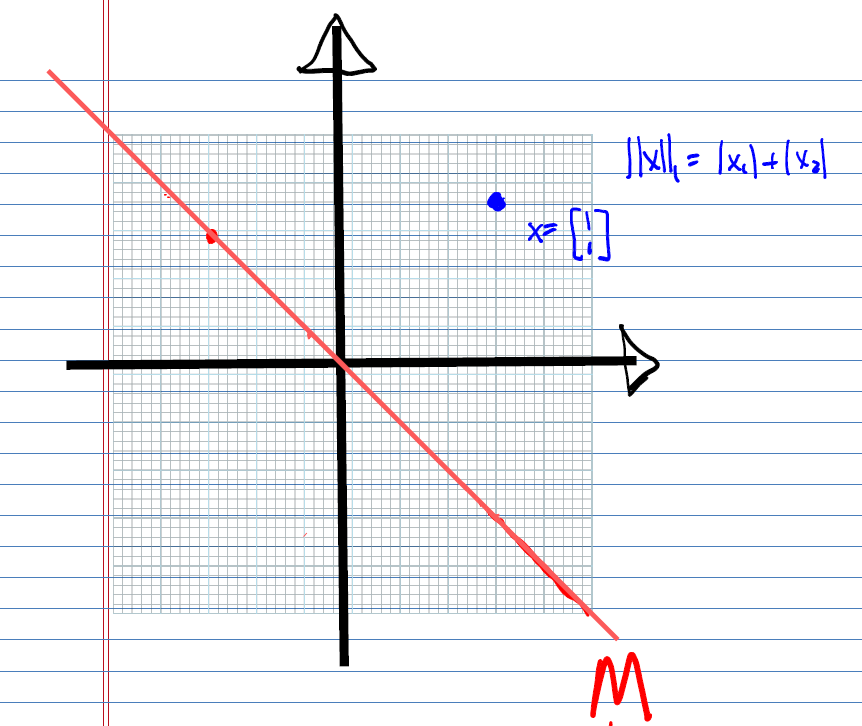
\includegraphics[width=0.7\columnwidth]{graphics/Chap03/NonUniqueMinimizingVector.png} }
    \caption[]{In HW, we'll introduce the concept of ``strict'' norms. The $|| \bullet ||_1$ is not strict and consequently, the minimum distance problem (or best approximation problem) does not have a unique answer. }
    \label{fig:NonUniqueMinimizingVector}
\end{figure} 

\begin{rem}
Figure~\ref{fig:NonUniqueMinimizingVector} shows an example having \textbf{nonunique solutions}. Indeed,  the set
$$S:= {\underset{y \in M}{\argmin}} \|x-y\|_1$$
contains an uncountable number of elements. Specifically, every element of
$$S=\left\{ \begin{bmatrix} x_1 \\ x_2 \end{bmatrix}~\big|~ x_2=-x_1, |x_1|\le 1 \right\} $$
is a minimizing vector for $x=[1~~~1]^\top$. That is, 
$$\forall~\widehat{x} \in S,~ ||x - \widehat{x}||_1 = 2 = \inf_{m \in M} ||x-m||_1.$$
To see this, you need to show that, $\forall~\widehat{x} \in S,$
\begin{align*}||x - \widehat{x}||_1 &= |1 - \hat{x}_1| + | 1 + \hat{x}_1|, ~-1 \le  \hat{x}_1 \le 1\\
& = (1 - \hat{x}_1)  +  ( 1 + \hat{x}_1) \\
&=2
\end{align*}
\end{rem}


\begin{exercise} Consider $(\real^n, \real)$ with the $p$-norm. Show that for all $x\in \real^n$, 
$$\lim_{p \to \infty}||x||_p= ||x||_{\rm max}. $$
\end{exercise}

\textbf{Hints:} (i) Prove the result when $||x||_{\rm max} =1$. (ii) When $x\neq 0$, consider $\bar{x} = x /||x||_{\rm max}$. (iii) For any non-negative real number $a$, $\lim_{p\to \infty} \sqrt[^p]{a} =1$.



\section{Inner Product Spaces}

\begin{recall}
For $z = \alpha + j\beta \, \in \mathbb{C}$, $\alpha, \beta \in\real$, we define $\mathrm{Re}\{z\}:=\alpha$ and  $\mathrm{Im}\{z\}:=\beta$. Note that $\mathrm{Im}\{z\}\in \real$. The complex conjugate of $z$ is $\overline{z} := \alpha -  j\beta$ and $|z| := \sqrt{\ z \cdot \overline{z}~ }= \sqrt{\alpha^2 + \beta^2}$.  Note that $z \in \real \iff (z = \overline{z}) \iff (\mathrm{Im}\{z\}=0)$.  For any complex number $z$, $\mathrm{Re}\{z\} \le |z|$. Finally, $ z = 0 \iff \overline{z} = 0 \iff |z|=0$.
\end{recall}

\begin{definition}
    Let $(\mathcal{X}, \mathbb{C})$ be a vector space. A function $\langle \cdot \, , \cdot \rangle: \mathcal{X} \times \mathcal{X} \rightarrow \mathbb{C}$
is an inner product if
    \begin{enumerate}
    \renewcommand{\labelenumi}{(\alph{enumi})}
        \setlength{\itemsep}{.1cm}
        \item $\langle a, b\rangle = \overline{\langle b, a\rangle}$.
        \item $\langle \alpha_1 x_1 + \alpha_2 x_2, y \rangle = \alpha_1 \langle x_1, y \rangle + \alpha_2 \langle x_2, y \rangle$, linear in the left argument. Some books place the linearity on the right side. 
        \item $\langle x, x \rangle \, \ge \, 0$ for any $x \in \mathcal{X}$, and $\langle x, x \rangle\,=\, 0$ $\iff$ $x = 0$. (See below: $\langle x, x \rangle$ is a real number and therefore it can be compared to 0.)
    \end{enumerate}
     
\end{definition}

\begin{rem} \mbox{ }
 \begin{enumerate}
        \item $\langle x, x \rangle\, =\, \overline{\langle x, x \rangle}$, by (a) and hence, $\langle x, x \rangle$ is always a real number.
        \item If the vector space is defined as $(\mathcal{X},\real)$, replace (a) with $(\text{a}^{'})$ $\langle a, b \rangle \, =\, \langle b, a \rangle$
        \item What about linear combinations on the right side? From (a) and (b)
        \begin{align*}
        \langle x, \beta_1 y_1 + \beta_2 y_2 \rangle &= \overline { \langle \beta_1 y_1 + \beta_2 y_2 ,  x\rangle }\\
        & =\overline {  \beta_1 \langle y_1 ,  x\rangle +  \beta_2  \langle y_2  ,  x\rangle }\\
        & =\overline{ \beta_1} ~~\overline{ \langle y_1 ,  x\rangle}  + \overline{ \beta_2}~~  \overline{ \langle y_2  ,  x\rangle }\\
         & =\overline{ \beta_1} ~\langle x, y_1 \rangle  + \overline{ \beta_2}  ~ \langle x,  y_2 \rangle 
        \end{align*}
        \item If the field is the real numbers, then the above reduces to $ \langle x, \beta_1 y_1 + \beta_2 y_2 \rangle = \beta_1 ~\langle x, y_1 \rangle  +  \beta_2  ~ \langle x,  y_2 \rangle  $
    \end{enumerate}

\end{rem}
   


\begin{example} Common inner products:
    \begin{enumerate}
        \renewcommand{\labelenumi}{(\alph{enumi})}
        \setlength{\itemsep}{.1cm}
        \item $(\mathbb{C}^n, \mathbb{C})$, $\langle x, y\rangle\, :=\, x^\top \overline{y}\, =\, \sum\limits_{i=1}^{n}x_i\overline{y_i}$.
        \item $(\real ^n,\real)$, $\langle x, y\rangle\, :=\, {x^\top }{y}\, =\, \sum\limits_{i=1}^{n}{x_i}{y_i}$.
        \item $\mathcal{F} =\real$, $\mathcal{X} = \{A\, |\, n\times m \,\, \text{real matrices} \}$, $\langle A, B\rangle\, :=\, \tr(AB^\top )\, = \, \tr(A^\top  B)$.
        \item $\mathcal{X} = \{ f: [a, b]\rightarrow\real , \text{$f$ continuous}\}$, $\mathcal{F} =\real$, $\langle f, g\rangle\, :=\,  \int_a^b \! f(t)g(t) \, \mathrm{d}t$.
    \end{enumerate}

\end{example}

\begin{thm}
    \textbf{(Cauchy-Schwarz Inequality)} Let $(\mathcal{X}, \mathcal{F}, \langle \cdot\,,\cdot \rangle)$ be an inner product space, with $\mathcal{F}$ either $\real $ or $\mathbb{C}$. Then, for all $x, y\in \mathcal{X}$
    \begin{equation*}
        |\langle x, y\rangle|\, \le\, {\langle x, x \rangle}^{1/2}\langle y, y \rangle ^{1/2}.
    \end{equation*}
\end{thm}

\textbf{Proof:} We will first do the proof for $\mathcal{F} =\real$.  We note that if $y = 0$, the result is clearly true. Hence, we assume $y \neq 0$ and let $\lambda \in\real$ be a scalar that is to be chosen. Then,
    \begin{align*}
        0\, & \le ||x - \lambda y||^2 \\
        &=  \langle x-\lambda y,\, x-\lambda y \rangle\\
        &=\langle x,\, x-\lambda y \rangle - \lambda\langle y,\, x-\lambda y\rangle\\
        &=\langle x, x\rangle - \lambda\langle x, y\rangle - \lambda\langle y, x\rangle +
        \lambda^2 \langle y, y\rangle \\
        &=\langle x, x\rangle - 2\lambda\langle x, y\rangle + \lambda^2\langle y,y\rangle.
    \end{align*}

We'll now make a choice for $\lambda$ that minimizes $\langle x, x\rangle - 2\lambda\langle x, y\rangle + \lambda^2\langle y,y\rangle$. Taking the derivative with respect to $\lambda$ and setting it equal to zero yields $\lambda = \langle x, y \rangle/\langle y, y \rangle$. In case you are curious whether this is a max or min, note that $\langle y, y \rangle >0$ because $y \neq 0$.\\

Substituting in this value for $\lambda$ gives
    \begin{align*}
        0& \le \min \limits_{\lambda \in \real}~~{\langle x-\lambda y, x-\lambda y\rangle} \\
        & = \left. \langle x- \lambda y, x- \lambda y \rangle \right|_{ \lambda = \langle x, y \rangle/ \langle y, y \rangle } \\
        &=\langle x,x\rangle - 2{|\langle x, y\rangle|}^2/\langle y,y \rangle + {|\langle x, y \rangle|}^2/{\langle y, y\rangle}\\
        &=\langle x,x\rangle - |\langle x,y\rangle|^2/\langle y, y\rangle \\
        & \Downarrow \\
      0  &\le  \langle x,x\rangle \cdot \langle y, y\rangle -|\langle x,y\rangle|^2
    \end{align*}
    Therefore, we can conclude that $|\langle x,y\rangle|^2\leq\langle x,x\rangle\langle y,y\rangle$ $\implies$ $|\langle x,y\rangle|\leq\langle x,x\rangle^{1/2}\langle y,y\rangle^{1/2}$ and the proof is done.\\

We quickly outline the steps for $\mathcal{F}=\cp$. Because the inner product of a vector with itself is always a non-negative real number, for all scalars $\lambda \in \cp$,
$$0 \le ~ \langle x-\lambda y, x-\lambda y \rangle   = \langle x,x \rangle   - \lambda \langle  y, x \rangle   - \overline{\lambda} \langle  x, y \rangle   + |\lambda|^2 \langle y,y \rangle  .$$
 For the particular choice $\lambda = \frac{\langle x, y \rangle  }{\langle y,y \rangle  }$, direct calculation shows
$$0 \le~ \langle x,x \rangle   - \frac{|\langle x,y \rangle  |^2}{\langle y,y \rangle  }, $$
which gives
$$|\langle x,y \rangle  | \le \sqrt{\langle x,x \rangle   \langle y,y \rangle  } = \langle x,x \rangle  ^{1/2} \cdot \langle y,y \rangle  ^{1/2},$$ 
and the proof is done. \\

\textbf{Note:} With the above choice of $\lambda$, we have 
$$\lambda \cdot \langle  y, x \rangle   = \frac{|\langle x,y \rangle  |^2}{\langle y,y \rangle  },~~  \overline{\lambda} \cdot \langle  x, y \rangle   =  \frac{|\langle x,y \rangle  |^2}{\langle y,y \rangle  }, \text{ and } |\lambda|^2 \cdot \langle y,y \rangle   =\frac{|\langle x,y \rangle  |^2}{\langle y,y \rangle  }. $$
    
    \Qed
    
\vspace*{.2cm}

\begin{cor}
Let $(\mathcal{X}, \mathcal{F}, \langle \cdot\,,\cdot \rangle)$ be an inner product space, with $\mathcal{F}$ either $\real $ or $\mathbb{C}$. Then, $$\|x\| :=  \langle x,x \rangle ^{1/2} = \sqrt{ \langle x,x \rangle }$$
is a \textbf{norm}.
\end{cor} 

\textbf{Proof:} As before,  for clarity of exposition, we first assume $\mathcal{F} =\real$. We will only check the triangle inequality $\|x+y\| \leq \|x\| +\|y\|$, which is equivalent to showing $ \|x+y\|^2 \leq \|x\|^2 + \|y\|^2 + 2\|x\| \cdot \|y\|$. The other parts are left as an exercise.

    \begin{align*}
               \|x+y\|^2 &:=  \langle x+y,x+y \rangle  \\
        &=  \langle x,x+y \rangle  +  \langle y, x+y \rangle  \\
        &=  \langle x,x \rangle  + \langle x,y \rangle  +  \langle y,x \rangle +  \langle y,y \rangle  \\
        &= \|x\|^2 + \|y\|^2 +2 \langle x,y \rangle  \\
        &\leq \|x\|^2 + \|y\|^2 + 2\left| \langle x,y \rangle \right| \\
        &\leq \|x\|^2 + \|y\|^2 + 2\|x\| \cdot \|y\|\, 
    \end{align*}
    where the last step uses the Cauchy-Schwarz inequality.  \\
    
    We'll now quickly do the changes required to handle $\mathcal{F} = \cp$. The triangle inequality is
$
	\| x + y \| \leqslant \| x \| + \| y \|,
$ which is equivalent to showing $
	\| x + y \|^2 \leqslant \| x \|^2 + 2 \| x \| \, \| y \| + \| y \|^2.
$
Brute force computation yields,
\begin{align*}
	\| x + y \|^2 &= \langle x+y,x+y \rangle   \\
	&= \langle x,x+y \rangle   + \langle y,x+y \rangle  \\
&= \overline{\langle x+y,x \rangle  } + \overline{\langle x+y,y \rangle  }\\
&= \overline{\langle x,x \rangle   + \langle y,x \rangle  } + \overline{\langle x,y \rangle   + \langle y,y \rangle  }\\
	&= \langle x,x \rangle   +  \langle x,y \rangle   +   \overline{\langle x,y \rangle  }+ \langle y,y \rangle   \\
	&= \| x \|^2 + \| y \|^2 + 2 \mathrm{Re}\{ \langle x,y \rangle  \}
\end{align*}
where $\mathrm{Re}\{ \langle x,y \rangle  \}$ denotes the real part of the complex number $\langle x,y \rangle  $. However, for any complex number $\alpha$, $\mathrm{Re}\{\alpha \} \le | \alpha|$, and thus we have
\begin{align*}
\| x + y \|^2 &= \| x \|^2 + \| y \|^2 + 2 \mathrm{Re}\{ \langle x,y \rangle  \} \\
	&\leqslant \| x \|^2 + \| y \|^2 +
		 2 |\langle x,y \rangle  | \\
	&\leqslant \| x \|^2 + \| y \|^2
		+ 2 \|x \| \|y\|,
\end{align*}
where the last inequality is from the Cauchy-Schwarz Inequality.
    
    
    \Qed
    
    \vspace*{.2cm}
    

\begin{definition}
    Orthogonal and orthonormal vectors.
\begin{enumerate}
        \renewcommand{\labelenumi}{(\alph{enumi})}
        \setlength{\itemsep}{.1cm}
    \item Two vectors $x$ and $y$ are \textbf{orthogonal} if $ \langle x,y \rangle =0$. \textbf{Notation:} $x \perp y$
    \item \textbf{A set of vectors $S$ is orthogonal} if $$\forall x \text{,} y \in S \text{,} x \neq y \implies \langle x,y \rangle =0 \mbox{ (i.e. $ x \perp y$)}$$
    \item If in addition, $\|x\|=1$ for all $x \in S$, then $S$ is an \textbf{orthonormal set}.
\end{enumerate}

\end{definition}


\begin{rem}
 For $x \neq 0, \frac{x}{\|x\|}$ has norm 1, because 
    $\left \lVert \frac{x}{\|x\|}\right\rVert = \left| \frac{1}{\|x\|}\right| \cdot \|x\|=\frac{1}{\|x\|}\cdot \|x\|=1$.
\end{rem}

 \begin{thm}
     \textbf{(Pythagorean Theorem)} If $x \perp y$, then
    $$\|x+y\|^2 = \|x\|^2+ \|y\|^2.$$\\
 \end{thm}

\textbf{Proof:} From the proof of the triangle inequality,
    \begin{align*}
        \|x+y\|^2 &= \|x\|^2+ \|y\|^2+2 \langle x,y \rangle.
    \end{align*}
    Once we note that $ \langle x,y \rangle = 0$  because $ x \perp y$, we are done. 
    
\Qed

 
 \section{Gram Schmidt Process}
 
\begin{prop}
 \textbf{(Recursion Step Gram Schmidt Process)} Let $({\cal X, F}, \langle \cdot, \cdot \rangle  )$ be  an inner product space, $\{ y^1, \cdots, y^k\}$ a linearly independent set, and 
$\{ v^1, \cdots, v^{k-1} \}$ an orthogonal set satisfying
  \begin{equation}
 \label{eq:gramSchmidtStepkminus1}
 \spanof{ v^1, \cdots, v^{k-1} } = \spanof{ y^1, \cdots, y^{k-1} } .
  \end{equation}
 Define
 \begin{equation}
 \label{eq:gramSchmidtRecursion}
	v^k = y^k - \sum_{j=1}^{k-1}
	\frac{\langle y^k,v^j \rangle  }{\| v^j \|^2} \cdot v^j		
\end{equation}
where $ \| v^j \|^2 = \langle v^j,v^j \rangle  $. Then, $\{ v^1, \cdots, v^{k} \}$ is orthogonal and
 \begin{equation}
 \label{eq:gram_schmidt}
\spanof{ v^1, \cdots, v^{k} } = \spanof{y^1, \cdots, y^{k}}.
 \end{equation}

\end{prop}

\textbf{Proof:} We first note that from \eqref{eq:gramSchmidtStepkminus1}, $v^i \neq 0$  for $1 \le i \le k-1$. Next, the orthogonality of $\{ v^1, \cdots, v^{k} \}$ is essentially by construction. To see this, we write
 $$v^k = y^k - \sum_{i=1}^{k-1} a_{ki}v^i	 $$
 and then check that $\langle v^k,v^j \rangle  =0$ for $1 \le j \le  k-1$  if, and only if,
 $$ a_{kj}=	\frac{\langle y^k,v^j \rangle  }{\| v^j \|^2} .$$
 Indeed,  
 $$ \langle  v^i, v^j  \rangle   = \begin{cases}
 0 & j \neq i, 1 \le i,j \le k-1 \\
|| v^i|| ^2 & i = j,
 \end{cases} $$
and hence 
$$0 = \langle v^k, v^j \rangle    = \langle y^k, v^j \rangle   - \sum_{i=1}^{k-1} a_{ki} \langle v^i, v^j \rangle   = \langle y^k, v^j \rangle   -  a_{kj} \langle v^j, v^j \rangle  	=  \langle y^k, v^j \rangle   -  a_{kj} ||v^j||^2. $$ 

 We next show that $y^k \in \spanof{ v^1, \cdots, v^k }$ and $v^k \in \spanof{ y^1, \cdots, y^k }$.\\

From \eqref{eq:gramSchmidtRecursion},
\[
	y^k = v^k + \sum_{j=1}^{k-1}
	\frac{\langle y^k,v^j \rangle  }{\| v^j \|^2} \cdot v^j  \implies 
	y^k \in
		\spanof{ v^1, \cdots, v^k }.
\]
Left to show: $v^k \in \spanof{ y^1, \cdots, y^k }$. By hypothesis,
\[
	v^j \in \spanof{ y^1, \cdots, y^{k-1} }
		\mbox{ for all } 1 \leqslant j \leqslant k-1,
\]
so
\[
	\sum_{j=1}^{k-1}
	\left( \frac{\langle v^j,y^k \rangle  }{\| v^j \|^2} \right) v^j \
		\in \ \spanof{ y^1, \cdots, y^{k-1} } \
		\subset \ \spanof{ y^1, \cdots, y^k }.
\]
Clearly, $y^k \in \spanof{ y^1, \cdots, y^k }$. Putting these two facts together, 
\[
 v^k = y^k - \sum_{j=1}^{k-1}
	\left( \frac{\langle v^j,y^k \rangle  }{\| v^j \|^2} \right) v^j \
		\in \ \spanof{ y^1, \cdots, y^k }
\]
because $\spanof{ y^1, \cdots, y^k }$ is a subspace. 
\Qed

\vspace*{.2cm}

\begin{definition}
\label{def:ClassicalGS}
The \textbf{Gram-Schmidt Process} consists of initialing \eqref{eq:gramSchmidtStepkminus1} with $v^1 = y^1$ and then applying \eqref{eq:gramSchmidtRecursion} recursively. When implementing the algorithm in code, it is quite easy to normalize the vectors as you go, as in the following pseudocode: 
\begin{lstlisting}[language=Julia,style=mystyle]
# Given {y1, ..., yn} linearly independent
# Produce {v1, ..., vn} orthonormal such that
# span{v1, ... vk} = span{y1, ..., yk}
v1 = y1
v1=v1/norm(v1)
for k = 2 : n
vk = yk
    for j = 1 : k - 1
        vk = vk - < yk, vj > 
    end
    vk = vk/norm(vk)
end
\end{lstlisting}
    
\end{definition} 
% \textbf{Output}
% \begin{verbatim}
% 1×5 Matrix{Float64}:
%  1.0  -2.0  4.0  8.1  1.41421
% \end{verbatim}

\begin{example} Given the following data in $(\real^3,\real)$, 
\begin{gather*}
	\{ y^1, y^2, y^3 \} = \left\{
		\left[ \begin{array}{c} 1 \\ 1 \\ 0 \end{array} \right],
		\left[ \begin{array}{c} 1 \\ 2 \\ 3 \end{array} \right],
		\left[ \begin{array}{c} 0 \\ 1 \\ 1 \end{array} \right]
		\right\},
\end{gather*}
and inner product $<p,q> := p^T q = \sum_{i=1}^3 p_i q_i$, apply Gram-Schmidt to produce an orthogonal basis. Normalize to produce an orthonormal basis.
\end{example}

\textbf{Solution:}
	\begin{align*}
		v^1 &= y^1 = \left[ \begin{array}{c} 1 \\ 1 \\ 0 \end{array} \right]\\
		\quad \| v^1 \|^2 &= (v^1)^T v^1 = 2 ;\\
		\\
		v^2	&= y^2 - \frac{<v^1,y^2>}{\| v^1 \|^2} v^1 \\
		&= \left[ \begin{array}{c} 1 \\ 2 \\ 3 \end{array} \right]
		- \underbrace{%
		   \left[ \begin{array}{ccc} 1 & 1 & 0 \end{array} \right]
		   \left[ \begin{array}{c} 1 \\ 2 \\ 3 \end{array} \right]%
		   }_{3}
		\frac{1}{2}
		   \left[ \begin{array}{c} 1 \\ 1 \\ 0 \end{array} \right]
		= \left[ \begin{array}{r}
			- \frac{1}{2} \medskip \\ \frac{1}{2} \medskip \\ 3
			\end{array} \right] \\
		\| v^2 \|^2 &= 9 \frac{1}{2} = \frac{19}{2} ;\\
		\\
		v^3	&= y^3 - \frac{<v^1,y^3>}{\| v^1 \|^2} v^1
			- \frac{<v^2,y^3>}{\| v^2 \|^2} v^2 \\
		&= \left[ \begin{array}{c} 0 \\ 1 \\ 1 \end{array} \right]
		- \underbrace{%
		   \left[ \begin{array}{ccc} 1 & 1 & 0 \end{array} \right]
		   \left[ \begin{array}{c} 0 \\ 1 \\ 1 \end{array} \right]%
		   }_{1}
		\frac{1}{2}
		   \left[ \begin{array}{c} 1 \\ 1 \\ 0 \end{array} \right]
		- \underbrace{%
		   \left[ \begin{array}{ccc}
			-\frac{1}{2} & \frac{1}{2} & 3 \end{array} \right]
		   \left[ \begin{array}{c} 0 \\ 1 \\ 1 \end{array} \right]%
		   }_{3\frac{1}{2}}
		\frac{1}{\frac{19}{2}}
		   \left[ \begin{array}{r}
			-\frac{1}{2} \medskip \\ \frac{1}{2} \medskip \\ 3 \end{array} \right] \\
		&= \left[ \begin{array}{c} 0 \\ 1 \\ 1 \end{array} \right]
		- \left[ \begin{array}{c}
			\frac{1}{2} \\ \frac{1}{2} \\ 0 \end{array} \right]
		- \left[ \begin{array}{r}
			-\frac{7}{38} \medskip \\ \frac{7}{38} \medskip \\ \frac{21}{19}
			\end{array} \right]
		= \left[ \begin{array}{r}
			-\frac{6}{19} \medskip \\ \frac{6}{19} \medskip \\ -\frac{2}{19}
			\end{array} \right].
	\end{align*}

\textbf{Normalize to obtain Orthonormal Basis:}often useful to do this, but never fun to do by hand.\\
	\begin{align*}
		\tilde{v}_1 &= \frac{v^1}{\| v^1 \|} = \left[ \begin{array}{c} \frac{1}{\sqrt{2}} \medskip \\ \frac{1}{\sqrt{2}} \medskip \\ 0 \end{array} \right]\\
		\tilde{v}_2 &= \frac{v^2}{\| v^2 \|} = \left[ \begin{array}{r} \frac{-1}{\sqrt{38}} \medskip \\ \frac{1}{\sqrt{38}} \medskip \\ 3\sqrt{\frac{2}{19}} \end{array} \right]\\
		\tilde{v}_3 &= \frac{v^3}{\| v^3 \|} = \frac{19}{\sqrt{76}} \left[ \begin{array}{r} -\frac{6}{19} \medskip \\ \frac{6}{19} \medskip \\ -\frac{2}{19}
			\end{array} \right]\\
	\end{align*}
\Qed

\begin{example} Given the real vector space $C[0,1] = \{ f:[0,1] \rightarrow \real \mid f~~\mbox{continuous} \}$, inner product $<f,g> := \int_0^1 f(\tau) g(\tau) d\tau$, and 
	$\{ y^1, y^2, y^3 \} = \{ 1, t, t^2 \}$, apply Gram-Schmidt to produce an orthogonal basis for $\spanof{ 1, t, t^2}$.

\end{example}

\textbf{Solution:}

	\begin{align*}
		v^1 &= y^1 = 1\\
		\qquad \| v^1 \|^2 &= \int_0^1 (1)^2 d\tau = 1 ;\\
		\\
		v^2	&= y^2 - \frac{<v^1,y^2>}{\| v^1 \|^2} v^1 \\
		&= t - \underbrace{%
			\int_0^1 1 \cdot \tau d\tau%
			}_{\frac{1}{2}} \cdot \frac{1}{1} \cdot 1
		= t - \frac{1}{2} \\
		\| v^2 \|^2 &= \int_0^1 (\tau - \frac{1}{2})^2 d\tau = \frac{1}{12} ;\\
		\\
		v^3	&= y^3 - \frac{<v^1,y^3>}{\| v^1 \|^2} v^1
		- \frac{<v^2,y^3>}{\| v^2 \|^2} v^2 \\
		&= t^2 - \underbrace{%
			\int_0^1 1 \cdot \tau^2 d\tau%
			}_{\frac{1}{3}} \cdot \frac{1}{1} \cdot 1
		- \underbrace{%
			\int_0^1 (\tau - \frac{1}{2}) \tau^2 d\tau%
			}_{\frac{1}{12}} \left( \frac{1}{\frac{1}{12}} \right)
				\Bigl( t - \frac{1}{2} \Bigr) \\
		&= t^2 - \frac{1}{3} - \Bigl( t - \frac{1}{2} \Bigr) \\
		&= t^2 - t + \frac{1}{6}.
	\end{align*}
	\Qed

\begin{example}
Doing inner products on $C[a,b]$ in MATLAB
% \begin{alltt}
% >> clear *
% >> syms t % declare to be a symbolic variable

% >> % INT(S,a,b) is the definite integral of S with respect to
%   % its symbolic variable from a to b.  a and b are each
%   % double or symbolic scalars.

% >> y1=1+0*t; % Otherwise MATLAB will not treat y1 as a 
%             %trivial function of the symbolic variable 
% >> y2=t;
% >> y3=t^2;

% % Start the G-S Procedure. Here we assume C[0,1], that is
% % C[a,b], with [a,b]=[0,1]

% >> v1=y1
% >> v2=y2-int(v1*y2,0,1)*v1/int(v1^2,0,1)
% >> v3=y3-int(v1*y3,0,1)*v1/int(v1^2,0,1)-
% int(v2*y3,0,1)*v2/int(v2^2,0,1)

% % Next, normalize to length one

% >> v1_tilde=v1/int(v1^2,0,1)^.5
% >> v2_tilde=simplify( v2/int(v2^2,0,1)^.5 )
% >> v3_tilde=simplyfy(v3/int(v3^2,0,1)^.5)
% \end{alltt}

\begin{lstlisting}[language=Julia,style=mystyle]
>> clear *
>> syms t % declare to be a symbolic variable

>> % INT(S,a,b) is the definite integral of S with respect to
   % its symbolic variable from a to b.  a and b are each
   % double or symbolic scalars.

>> y1=1+0*t; % Otherwise MATLAB will not treat y1 as a 
            %trivial function of the symbolic variable 
>> y2=t;
>> y3=t^2;

% Start the G-S Procedure. Here we assume C[0,1], that is
% C[a,b], with [a,b]=[0,1]

>> v1=y1
>> v2=y2-int(v1*y2,0,1)*v1/int(v1^2,0,1)
>> v3=y3-int(v1*y3,0,1)*v1/int(v1^2,0,1)-
int(v2*y3,0,1)*v2/int(v2^2,0,1)

% Next, normalize to length one

>> v1_tilde=v1/int(v1^2,0,1)^.5
>> v2_tilde=simplify( v2/int(v2^2,0,1)^.5 )
>> v3_tilde=simplyfy(v3/int(v3^2,0,1)^.5)
\end{lstlisting}
\textbf{Output} 
\begin{verbatim}
v1=1
v2=t-1/2
v3=t^2+1/6-t

v1_tilde=1
v2_tilde=(t-1/2)*12^(1/2)
v3_tilde=(6*t^2+1-6*t)*5^(1/2)
 \end{verbatim}
 
 \end{example}

\begin{rem}
\label{rem:ModifiedGramSchmidt} \textbf{(Round-off Errors Affect Classical Gram-Schmidt)}
The classical Gram-Schmidt Process in Definition~\ref{def:ClassicalGS} is straightforward to understand, which is why it is taught in courses. Unfortunately, it behaves poorly under the round-off error that occurs in digital computations! Here is a standard example:
    \begin{equation*}
        u_1=\left[\begin{matrix} 1 \\ \varepsilon \\ 0 \\ 0 \end{matrix}\right],
        u_2=\left[\begin{matrix} 1 \\ 0 \\ \varepsilon \\ 0 \end{matrix}\right],
        u_3=\left[\begin{matrix} 1 \\ 0 \\ 0 \\ \varepsilon \end{matrix}\right],
        \varepsilon>0
    \end{equation*}
Let $\{e_1,e_2,e_3,e_4\}$ be the standard basis vectors corresponding to the columns of the $4 \times 4$ identity matrix. We note that
    \begin{align*}
        u_2 &= u_1+\varepsilon(e_3-e_2)\\
        u_3 &= u_2+\varepsilon(e_4-e_3)
    \end{align*}
    and thus, for $\epsilon \neq 0,$
    \begin{align*}
        \spanof{u_1,u_2}&=\spanof{u_1,(e_3-e_2)}\\
        \spanof{u_1,u_2,u_3}&=\spanof{u_1,(e_3-e_2),(e_4-e_3)}
    \end{align*}
\end{rem}


\begin{example}
Hence, Gram-Schmidt applied to $\{u_1,u_2,u_3\}$ and $\{u_1,(e_3-e_2),(e_4-e_3)\}$ should ``theoretically'' produce the same orthonormal vectors. To check this, we go to MATLAB, and for $\varepsilon=0.1$, we do indeed get the same results. You can verify this yourself. However, with $\varepsilon=10^{-8}$,
\begin{align*}
    Q_1 &= \left[ \begin{array}{rrr}
  1.0000     &    0.0000     &  0.0000  \\
    0.0000 &  -0.7071  & -0.7071 \\
        0.0000  &   0.7071   &      0.0000  \\
        0.0000   &      0.0000  &  0.7071
    \end{array} \right] \\
    Q_2&=\left[ \begin{array}{rrr}
  1.0000     &    0.0000     &  0.0000  \\
    0.0000 &  -0.7071  & -0.4082 \\
        0.0000  &   0.7071   &      -0.4082  \\
        0.0000   &      0.0000  &  0.8165
    \end{array} \right] 
    \end{align*}
where $$Q_1=\begin{bmatrix} \frac{v_1}{\| v_1 \|} & \frac{v_2}{\| v_2 \|} & \frac{v_3}{\| v_3 \|}\end{bmatrix}$$
has been computed with Classical-Gram-Schmidt for $\{u_1,u_2,u_3\}$ while $$Q_2=\begin{bmatrix} \frac{v_1}{\| v_1 \|} & \frac{v_2}{\| v_2 \|} & \frac{v_3}{\| v_3 \|}\end{bmatrix}$$
has been computed with Classical-Gram-Schmidt for $\{u_1,(e_3-e_2),(e_4-e_3)\}$. Hence we do NOT obtain the same result!
\end{example}



\begin{definition} \textbf{(Modified Gram-Schmidt)} has better numerical performance\\
for $k=1:n$\\
        \indent\hspace{4ex}$v_k=u_k$~~~\%copy over the vectors\\
        end \bigskip\\
        for $k=1:n$\\
        \indent\hspace{4ex}$v_k=\frac{v_k}{\|v_k\|}$ \medskip\\
        \indent\hspace{4ex}for $j=(k+1):n$  \medskip\\
        \indent\hspace{8ex}$v_j=v_j-(v_j \bullet v_k)v_k$  ~~~\%Makes $v_j$ orthogonal to  $v_k$\\
        \indent\hspace{4ex}end\\
        end\\
        At \textbf{Step k=1}, $v_1$ is normalized to length one, and then $v_2, \ldots, v_n$ are redefined to be orthogonal to $v_1$. At \textbf{Step k=2:}  $v_2$ is normalized to length one, and then $v_3, \ldots, v_n$ are redefined to be orthogonal to $v_2$. We note that they were already orthogonal to $v_1$.  At \textbf{Step k:}  $v_k$ is normalized to length one, and then $v_{k+1}, \ldots, v_n$ are redefined to be orthogonal to $v_k$. We note that they were already orthogonal to $v_1, \ldots, v_{k-1}$.    
\end{definition}
 
        
 \begin{example}
Hence, if Modified Gram-Schmidt is so great, when applied to $\{u_1,u_2,u_3\}$ and $\{u_1,(e_3-e_2),(e_4-e_3)\}$, it should produce the same orthonormal vectors and it does! To check this, we go to MATLAB for $\varepsilon=10^{-8}$ and obtain
\begin{align*}
    Q_1 &= \left[ \begin{array}{rrr}
  1.0000     &    0.0000     &  0.0000  \\
    0.0000 &  -0.7071  & -0.7071 \\
        0.0000  &   0.7071   &      0.0000  \\
        0.0000   &      0.0000  &  0.7071
    \end{array} \right] \\
    Q_2&=\left[ \begin{array}{rrr}
  1.0000     &    0.0000     &  0.0000  \\
    0.0000 &  -0.7071  & -0.7071 \\
        0.0000  &   0.7071   &      0.0000  \\
        0.0000   &      0.0000  &  0.7071
    \end{array} \right]
    \end{align*}
where $Q_1$ and $Q_2$ are defined above. \textbf{When one is equipped with the right Algorithm, the world is truly a marvelous place.}
  
  \end{example}
  
  \begin{rem}
Just to be perfectly clear, with perfect arithmetic (no rounding errors), Classical Gram-Schmidt and Modified Gram-Schmidt are equivalent. 
  \end{rem}
 
 \section{Projection Theorem and the Normal Equations}
 
\begin{lem} (called the Pre-Projection Theorem in Luenberger)
\label{lem:PreProjThm}
Let $\mathcal{X}$ be a finite-dimensional (real) inner product space, $M$ be a subspace of $\mathcal{X}$, and $x$ be an arbitrary point in $\mathcal{X}$.
    \begin{enumerate}
            \renewcommand{\labelenumi}{(\alph{enumi})}
        \setlength{\itemsep}{.1cm}
        \item If $\exists m_0 \in M $ such that $\|x-m_0\| \leq \|x-m\| \ \ \forall m \in M$, then $m_0$ is unique.
        \item A necessary and sufficient condition for $m_0$ to be a minimizing vector in $M$ is that the vector $x-m_0$ is orthogonal to $M$.
    \end{enumerate}
        
\end{lem}

\textbf{Remarks:}
    \begin{enumerate}
        \item[(a')] If $\exists m_0 \in M$ such that $\|x-m_0\| = d(x,M) = \underset{m \in M}{\text{inf}} \|x-m\|$, then $m_0$ is unique. [equivalent to (a)]
        \item[(b')] $\|x-m_0\| = d(x,M) \iff x-m_0 \perp M$. [equivalent to (b)]
    \end{enumerate}

\textbf{Proof:} We break the proof up into a series of claims.

\begin{claim}
If $m_0 \in M$ satisfies $\|x-m_0\| = d(x,M)$, then $x-m_0 \perp M$. 
\end{claim}
    \emph{Proof:} (By contrapositive) Assume $x-m_0 \not\perp M$. We will produce $m_1 \in M$ such that $\|x-m_1\| <  \|x-m_0\|$. Indeed, suppose $x-m_0 \not\perp M$. Then, $\exists m \in M$ such that $ \langle x-m_0, m \rangle  \neq 0$. We know $m \neq 0$, and hence we define 
    \begin{itemize}
        \item $\tilde{m} = \frac{m}{\|m\|} \in M$; 
        \item $\delta := \langle x-m_0, \tilde{m} \rangle  \neq 0$; and
        \item $m_1 = m_0 + \delta \tilde{m} \implies m_1 \in M$.
    \end{itemize}
The intuition behind the definition of $m_1$ is that $x-m_1$ is ``closer'' to being perpendicular to $M$ than is $x - m_0$, and hence it should follow that $||x - m_1|| < ||x-m_0||$.  To prove the latter point, we do a few computations:
        \begin{align*}
            \|x-m_1\|^2 &= \|x-m_0-\delta \tilde{m}\|^2 \\
            &=  \langle x-m_0-\delta \tilde{m}, x-m_0-\delta \tilde{m} \rangle  \\
            &=  \langle x-m_0,x-m_0 \rangle  -\delta \underbrace{\langle x-m_0,\tilde{m} \rangle}_\delta -\delta \underbrace{\langle \tilde{m},x-m_0 \rangle}_\delta  +\delta^2 \underbrace{\langle \tilde{m},\tilde{m} \rangle}_{=1}  \\
            &= \|x-m_0\|^2 -\delta^2 \\
            &< \|x-m_0\|^2
        \end{align*}
    because $\delta^2 >0$.  Hence, $\|x-m_1\|^2 <  \|x-m_0\|^2$ and therefore, $\|x-m_0\| \neq \underset{m \in M}{\inf  \|x-m\|}:= d(x,M)$.  \hfill   $\square$ 
   
 

\begin{claim}
 If $x-m_0 \perp M$, then $\|x-m_0\| = d(x,M)$ and $m_0$ is unique. 
\end{claim}
\emph{Proof:} Recall the Pythagorean Theorem:
    \begin{equation*}
        \|x+y\|^2=\|x\|^2+\|y\|^2 \mbox{ when } x \perp y
    \end{equation*}
    Let $m \in M$ be arbitrary and suppose $x-m_0 \perp M$. Then  $x-m_0 \perp  m_0-m$, and thus
    \begin{align*}
        \|x-m\|^2 &= \|x-m_0+\underbrace{m_0-m}_{\in M}\|^2 \\
        &= \|x-m_0\|^2 + \|m_0 - m\|^2.
    \end{align*}
    It follows that
    $$\underset{m \in M}{\text{inf}} \|x-m\|^2=\underset{m \in M}{\inf~ }\left( \|x-m_0\|^2 + \|m_0 - m\|^2 \right) = 
     \|x-m_0\|^2 + \underset{m \in M}{\inf~ } \|m_0 - m\|^2 =\|x-m_0\|^2. $$ 
The unique minimizer is $m_0$ because $ \|m_0 - m\|^2 =0$  only for $m=m_0$. \hfill $\square$ \\

The two claims complete the proof. 

\Qed

\begin{definition}
Let $({\cal X, F},  \langle \cdot,\cdot \rangle )$ be an inner product space, and $S \subset {\cal X}$ a \emph{subset} (does not have to be a subspace). 
$$S^{\perp}:= \{x \in {\cal X}|x \perp S\} = \{x \in {\cal X}|  \langle x,y \rangle =0 \textnormal{ for all }y \in S\}$$
is called \textbf{the orthogonal complement of $S$}.
\end{definition}

\begin{exercise} \mbox{ }
\begin{itemize}
    \item Show that $S^{\perp}$ is always a subspace. 
    \item If $M = \spanof{y^1, \ldots, y^k},$ show that $(x \in M^\perp) \iff \langle x,y^i \rangle =0, ~ 1 \le i \le k$.
\end{itemize}


\end{exercise}

\begin{prop}
\label{prop:DirectSum}
 Let $({\cal X, F}, \langle \cdot, \cdot \rangle )$ be a finite dimensional inner product space and $M$ a subspace of $\cal X$. Then, $${\cal X} = M \oplus M^{\perp}.$$
\end{prop}

\begin{rem}
Suppose that $V$ and $W$ are subspaces of $\cal X$. Then $V+W:=\{ x\in {\cal X}~|~ x = v + w, \text{ for some } v\in V, w \in W\}$. Because $V$ and $W$ are subspaces, $0\in V \cap W$ (the zero vector is in their intersection). If that is the only vector in the intersection, meaning $V \cap W = \{0\}$, the zero subspace, then we write $V \oplus W$, and it is called the \textbf{direct sum} of $V$ and $W$. What does the direct sum get you that an ordinary sum would not? You can show that $(x \in V \oplus W) \iff (\exists ~~\text{\bf unique } v \in V, w \in W \text{ such that } x = v+w).$ 
\end{rem}

\textbf{Proof:} If $x\in M\cap M^\perp$, then by the definition of $M^\perp$, $ \langle x,x \rangle =0$, which implies $x=0$. Hence, $M \cap M^{\perp} = \{0\}$. Next, we need to show that ${\cal X} = M + M^{\perp}$, that is, every $X\in {\cal X} $ can be written as a sum of a vector in $M$ and a vector in $M^\perp$.\\

Let $\{y^1, \ldots, y^k\}$ be a basis of $M$. By Corollary~\ref{cor:Complete2Basis},  it can be completed to a basis for $\cal X$, that is, $${\cal X} = \spanof{y^1, y^2, \ldots, y^k, y^{k+1}, \ldots, y^n} \text{ and } \{y^1, y^2, \ldots, y^k, y^{k+1}, \ldots, y^n \} \text{ is linearly independent}.$$
We can then apply Gram-Schmidt to produce orthonormal vectors $\{v^1, \ldots, v^k, v^{k+1}, \ldots, v^n\}$ such that $$\spanof{v^1, \ldots, v^k} = \spanof{y^1, \ldots, y^k} = M \text{ and } \spanof{v^1, \ldots, v^k, v^{k+1}, \ldots, v^n} ={\cal X}.$$
An easy calculation gives
    $$M^{\perp} = \spanof{v^{k+1}, \ldots, v^n}.$$
Indeed, suppose $x = \alpha_1 v^1 + \cdots + \alpha_k v^k + \alpha_{k+1} v^{k+1} + \cdots + \alpha_n v^n$. Then $x \in M^\perp \iff x \perp M \iff \langle x, v^i \rangle =0, 1 \leq i \leq k $. However, 
    \begin{align*}
        \langle x, v^i \rangle  &= \alpha_1  \langle v^1, v^i \rangle  + \cdots + \alpha_i  \langle v^i, v^i \rangle  + \cdots + \alpha_n  \langle v^n, v^i \rangle\\
        &= \alpha_i ~~~ (\text{because }  \langle v^j, v^i \rangle = 0, ~j \neq i, \text{ and } \langle v^i, v^i \rangle = 1)
    \end{align*}
    and therefore $x \perp M \iff \alpha_i = 0$, $1 \le i \le k$. This yields
$(x \in M^\perp) \iff (x = \alpha_{k+1} v^{k+1} + \cdots + \alpha_n v^n) \iff (x \in \spanof{v^{k+1}, \cdots, v^n})$. Therefore,
$$ M^{\perp} =\spanof{v^{k+1}, \ldots, v^n}.$$
\Qed


\begin{thm} 
\label{thm:ClassicalProjThm}
\textbf{(Classical Projection Theorem)}  Let $({\cal X}, \real)$ be a finite dimensional real inner product space and $M$ a subspace of $\cal X$. Then, $\forall x \in {\cal X}, \exists \textnormal{ unique }\widehat{x} \in M$ such that
    \begin{equation*}
        \|x - \widehat{x}\| = d(x, M) := \inf\limits_{m \in M} \|x - m\| =\min\limits_{m \in M} \|x - m\|,
    \end{equation*}
    where we can write $\min$ instead of $\inf$ because the infimum is achieved. Moreover, $\widehat{x} \in M$ is characterized by $x-\widehat{x} \perp M$.
        
\end{thm}

\textbf{Proof:} We only need to show that $\forall x \in {\cal X}$ there exists $\widehat{x} \in M$ such that $(x - \widehat{x}) \perp M$. This is because if such an $\widehat{x}$ exists,  Lemma~\ref{lem:PreProjThm}, the ``Pre-projection Theorem,'' already shows that it is unique and $ \|x - \widehat{x}\| = d(x, M)$. By Proposition~\ref{prop:DirectSum}, ${\cal X} = M \oplus M^{\perp}$. Therefore, there exist $\widehat{x} \in M$ and $m^\perp \in M^\perp$
such that
    $$x = \widehat{x} + m^\perp.$$
    Hence,
    $$x-\widehat{x} = m^\perp \in M^\perp \implies (x-\widehat{x}) \perp M.$$
    \Qed

\begin{rem}
You may have observed that ${\cal X} = M \oplus M^{\perp}$ also shows that $\widehat{x}$ is unique. While this is true, it is based on Proposition~\ref{prop:DirectSum}, which is true when ${\cal X}$ is a ``complete'' inner product space and $M$ is a ``closed'' subspace, properties that are automatically satisfied when ${\cal X}$ is finite dimensional. We will touch on these more subtle properties later when we do some basic Real Analysis.
\end{rem}


\begin{notation}
$\widehat{x} = \argmin d(x,M) = \argmin \limits_{m \in M} \|x - m\|.$
\end{notation}

Our next goal is to turn Theorem~\ref{thm:ClassicalProjThm} into a means to compute the best approximation value, $\widehat{x}$. By the Projection Theorem, $\widehat{x} $ exists and is characterized by $x-\widehat{x} \perp M$. We write
$$\widehat{x}= \alpha_1 y^1+ \alpha_2 y^2+ \cdots +\alpha_k y^k$$
and impose 
$$(x-\widehat{x} \perp M )\iff (x-\widehat{x} \perp y^i,~ 1 \le i \le k) \iff ( \langle x-\widehat{x},y^i \rangle =0,~ 1 \le i \le k) \iff (\langle \widehat{x},y^i \rangle = \langle x,y^i \rangle ~ 1 \le i \le k). $$

Then, 
\begin{align*}
\langle \widehat{x},y^i \rangle &= \langle x,y^i \rangle  ~ 1 \le i \le k \\
& \Updownarrow \\
\langle \alpha_1 y^1+ \alpha_2 y^2+\cdots +\alpha_k y^k, y^i \rangle  & =  \langle x,y^i \rangle ~ 1 \le i \le k  \\
& \Updownarrow \\
\alpha_1  \langle y^1,y^i \rangle +\alpha_2  \langle y^2,y^i \rangle + \cdots + \alpha_k  \langle y^k,y^i \rangle &=  \langle x,y^i \rangle ~ 1 \le i \le k  
\end{align*}

We now write these equations out in matrix form.
\begin{equation}
\label{eq:NormalEquations01}
    \begin{aligned}
    i=1 ~~~~& \alpha_1  \langle y^1,y^1 \rangle +\alpha_2  \langle y^2,y^1 \rangle + \cdots + \alpha_k  \langle y^k,y^1 \rangle =  \langle x,y^1 \rangle \medskip \\
    i=2 ~~~~& \alpha_1  \langle y^1,y^2 \rangle +\alpha_2  \langle y^2,y^2 \rangle + \cdots + \alpha_k  \langle y^k,y^2 \rangle =  \langle x,y^2 \rangle \\
   \vdots ~~~~~~~~ & \hspace{4cm} \vdots \\
    i=k~~~~& \alpha_1  \langle y^1,y^k \rangle +\alpha_2  \langle y^2,y^k \rangle + \cdots + \alpha_k  \langle y^k,y^k \rangle =  \langle x,y^k \rangle.
    \end{aligned}
\end{equation}


\begin{definition}
Equations~\ref{eq:NormalEquations01} are called the \textbf{Normal Equations}. The \textbf{Gram Matrix} is the $k \times k$ matrix $G_{ij}: =  \langle y^i,y^j \rangle$. The \textbf{Normal Equations} can also refer to 
\begin{equation}
\label{eq:NormalEquations02}
 G^\top \alpha = \beta
\end{equation}
where,
$$  \alpha:=\begin{bmatrix} \alpha_1 \\ \alpha_2 \\ \vdots \\ \alpha_k  \end{bmatrix}, ~  \beta:=\begin{bmatrix} \langle x,y^1 \rangle \\ \langle x,y^2 \rangle \\ \vdots \\ \langle x,y^k \rangle \end{bmatrix}=:\begin{bmatrix} \beta_1 \\ \beta_2 \\ \vdots \\ \beta_k  \end{bmatrix}, \text{ and } G:=G(y^1,\cdots , y^k):=\left[ \begin{array}{cccc}  \langle y^1,y^1 \rangle  &  \langle y^1,y^2 \rangle  & \cdots &  \langle y^1,y^k \rangle  \\  \langle y^2,y^1 \rangle  &  \langle y^2,y^2 \rangle  & \cdots &  \langle y^2,y^k \rangle \\ \vdots & \vdots && \vdots \\  \langle y^k,y^1 \rangle  &  \langle y^k,y^2 \rangle  & \cdots &  \langle y^k,y^k \rangle  \end{array}  \right].$$

\end{definition}

\begin{rem}
Because we are assuming $\cal F =\real  $,  $G_{ij}= \langle y^i,y^j \rangle = \langle y^j,y^i \rangle = G_{ji}$, and we therefore have $G=G^\top$. We'll show below that $\det(G) \neq 0$ if, and only if, $\{ y^1, y^2, \ldots, y^k\}$ is linearly independent. In this case, 
$$\widehat{x}= \alpha_1 y^1+ \alpha_2 y^2+ \cdots +\alpha_k y^k$$
with $G^\top \alpha = \beta$ is the best approximation to $x$ by an element in $M:=\spanof{ y^1, y^2, \ldots, y^k}$.
\end{rem}

\begin{prop} \textbf{(Invertibility of the Gram Matrix)}
\label{prop:GramInvertible}
Let $g(y^1,\ldots,y^k):=\det G(y^1,\ldots,y^k)$ be the determinant of the Gram Matrix. Then $g(y^1,\ldots,y^k) \neq 0 \iff \{ y^1, y^2, \ldots, y^k \}$ is linearly independent.
\end{prop} 

\textbf{Proof:} From our construction of the normal equations,  $G^\top \alpha = 0$ if, and only if
$$  \langle \alpha_1 y^1+ \alpha_2 y^2+\cdots +\alpha_k y^k, y^i \rangle  = 0, ~ 1 \le i \le k.$$
This is equivalent to
$$  \left( \alpha_1 y^1+ \alpha_2 y^2+ \cdots +\alpha_k y^k \right) \perp  y^i = 0,  ~ 1 \le i \le k,$$
which is equivalent to
$$  \left( \alpha_1 y^1+ \alpha_2 y^2+ \cdots + \alpha_k y^k \right) \perp  \textrm{span} \{ y^1, \cdots, y^k \}=:M $$
and thus
$$ \alpha_1 y^1+ \alpha_2 y^2+ \cdots + \alpha_k y^k  \in M^\perp.$$

Because $\alpha_1 y^1+ \alpha_2 y^2+\cdots +\alpha_k y^k \in M$, we have that
$$ \alpha_1 y^1+ \alpha_2 y^2+\cdots +\alpha_k y^k  \in M \cap M^\perp  =\{ 0 \}$$
and therefore
$ \alpha_1 y^1+ \alpha_2 y^2+\cdots +\alpha_k y^k  = 0.$ By the linear independence of
$\{ y^1, y^2, \ldots, y^k \}$, we deduce that $\alpha_i = 0, 1 \le i \le k$. 

\Qed

\begin{summary} \textbf{\emph{(The normal equations provide a systematic solution of our best approximation problem).}} Assume the set $\{ y^1,\ldots, y^k \}$ is linearly independent and $M:=\spanof{y^1,\cdots, y^k }$. Then
$\widehat{x} = \argmin d(x,M) =\argmin \limits_{m \in M} \|x - m\|$ if, and only if,
\begin{equation}
\begin{aligned}
\widehat{x} &= \alpha_1 y^1+ \alpha_2 y^2+ \cdots +\alpha_k y^k \\
G^\top \alpha &=\beta \\
G_{ij}&= \langle y^i,y^j \rangle \\
\beta_i &= \langle x,y^i \rangle.
\end{aligned} 
\end{equation}
What changes in each application of the normal equations is typically the inner product, $\langle \bullet , \bullet \rangle$. 
\end{summary}




\begin{tcolorbox}[title=\textbf{\Large Overdetermined Equations}]
Roughly speaking, a set of linear equations $Ax = b$ is \textbf{overdetermined} when $A$ has more rows than equations. Typically, in this case, there is no value of $x$ such that $Ax - b=0.$ Of course, if $b=0$ then $x=0$ is a solution, and more generally, there is a solution if, and only if, $b \in \colspanof{A}$, that is, $b$ can be written as a linear combination of the columns of $A$. When $b \not \in \colspanof{A}$, it makes sense to seek a ``best approximate solution'',  which we'll define to be a value $\widehat{x}$ that minimizes the norm of the error in the solution, that is, 
$$\widehat{x} := \argmin_{x} \| A x -b \|. $$

\textbf{Is there a difference between being overdetermined and having no exact solutions?} Yes. It's possible to be overdetermined and still have an exact solution when $b \in \colspanof{A}$. If the columns of $A$ are linearly independent, then 
$$Ax=b ~~\text{is overdetermined}~~\iff b \not \in \colspanof{A}.$$

\end{tcolorbox}

\begin{example}  
\label{ex:OverDetermined}
\textbf{\emph{(Overdetermined system of linear equations in $\real ^n$)}}
Consider $A \alpha=b,$ 
where $A=n \times m$ real matrix,  $n \geq m$, rank$(A)=m$ (columns of $A$ are linearly independent). From the dimension of $A$, we have that $\alpha \in \real^m , b \in\real^n$. Determine if there exists a ``best approximate solution'' using the Euclidean norm. 
\end{example}

\textbf{Solution ~1:} The \emph{Standard Problem Formulation and Solution} goes like this. We seek $\widehat{\alpha} \in \real^m $ such that $$\| A \widehat{\alpha}-b \|=\min_{\alpha \in\real^m} \| A \alpha -b \|,$$
where the norm is defined on the error, $e:=A \alpha - b \in \real^n$, namely
$\|e\| =\sqrt{\sum\limits_{i=1}^n (e_i)^2}.$ Hence, the problem is \\
$$\widehat{\alpha} =\argmin_{\alpha \in\real^m} \sqrt{(A \alpha -b)^\top (A \alpha -b)} = \argmin_{\alpha \in\real^m} (A \alpha -b)^\top (A \alpha -b).$$
The problem can be solved by ``completing the square'' or by applying vector calculus to compute the gradient, namely, 
$$\frac{\partial }{\partial \alpha }\left( (A \alpha -b)^\top (A \alpha -b) \right) = A^\top \cdot(A \alpha - b),$$
setting it to zero, and solving for $\alpha$. Once you convince yourself that $A^\top A$ is invertible, the solution is computed to be 
$$ A^\top \cdot(A  \widehat{\alpha} - b) = 0 \iff (A^\top A)\widehat{\alpha} = A^\top b \iff  \widehat{\alpha} = (A^\top A)^{-1} A^\top b.$$

\textbf{Solution ~2:} \emph{Our Problem Formulation and Solution:} The standard formulation puts all the emphasis on the $\alpha$ and misses that $A \alpha $ is a linear combination of the columns of $A$. The problem is calling for a linear combination of the columns of $A$ that best approximates the vector $b$.  We will therefore apply the normal equations \eqref{eq:NormalEquations02}, where the column span of $A$ is the subspace $M$ and $b$ is the vector $x \in \mathcal{X}$.\\

\textbf{Inner product space:} ${\cal X}=\real ^n$, ${\cal F}=\real$, $\langle x,y \rangle = x^T y= y^T x= \sum\limits_{i=1}^n x_i y_i \implies \|x\|^2= \langle x,x \rangle =\sum\limits_{i=1}^n |x_i|^2.$\\


Partition $A=\left[ \begin{array}{cccc} A_1 & A_2 & \cdots & A_m \end{array} \right]$ and define $\alpha = \left[ \begin{array}{cccc}\alpha_1 & \alpha_2 &  \cdots & \alpha_m \end{array} \right]^\top$, and note that
$$ A \alpha = \alpha_1 A_1 + \alpha_2 A_2 + \cdots + \alpha_m A_m.$$

\textbf{Seek:} $\widehat{x} = A \widehat{\alpha} \in \spanof{ A_1,A_2, \cdots, A_m } =: M$
such that  $\|\widehat{x}-b\|=d(b,M).$ By the Projection Theorem and the Normal Equations,
$$\widehat{x}=\widehat{\alpha}_1 A_1 +\widehat{\alpha}_2 A_2 + \cdots \widehat{\alpha}_m A_m $$
and $G^\top \widehat{\alpha}=\beta$, with
$$G_{ij}= \langle A_i,A_j \rangle =A_i ^\top A_j = [A^\top A]_{ij} \text{ and } \beta_i =  \langle A_i, b \rangle  =  A_i^\top b = [A^\top b]_i.$$
Hence, $G^\top = A^\top A$ and $\beta = A^\top b$. By  Proposition~\ref{prop:GramInvertible}, $G$ is invertible because the columns of $A$ are linearly independent. Therefore, we have that
$$\widehat{\alpha}=(A^\top A)^{-1} A^\top b.$$
\Qed

\begin{rem} Once we note that 
$$A^\top=\begin{bmatrix} A_1^\top \medskip \\ A_2^\top \medskip\\ \vdots \medskip\\ A_m^\top \medskip \end{bmatrix} \text{ when } A= \left[ \begin{array}{cccc} A_1 & A_2 & \cdots & A_m \end{array} \right]$$ 
The standard ``row times column'' definition of matrix multiplication gives that $(A^\top A)_{ij}=A^\top_i A_j$. Similarly, $(A^\top b)_i=A_i^\top b$. 
\end{rem}


\begin{definition} \textbf{(Orthogonal Projection Operator)} Let $\cal X$ be a finite dimensional (real) inner product space and $M$ a subspace of $\cal X$. For $x \in \cal X$ and $\widehat{x} \in M$. The Projection Theorem shows the TFAE:
\begin{enumerate}
\renewcommand{\labelenumi}{(\alph{enumi})}
    \item $x-\widehat{x}   \perp M $.

    \item $\exists m^\perp \in M^{\bot}$ such that  $ x=\widehat{x}  + m^\perp $.

    \item $ \|x-\widehat{x} \|=d(x,M)=\inf\limits_{m \in M} \|x-m\|$.
\end{enumerate}
A function $P$: ${\cal X}\to M$ by $P(x)=\widehat{x} $, where $\widehat{x} $ satisfies any one of (a), (b), or (c), is called the \textbf{Orthogonal Projection} of $\cal X$ onto $M$.
\end{definition}


\begin{exercise} Key properties of the \emph{orthogonal projection operator}.
\begin{itemize}
    \item The orthogonal projection operator $P$: ${\cal X}\rightarrow M$ is a linear operator.
    \item  Let $\{v^1,\ldots ,v^k\}$ be an \emph{orthonormal basis} for $M$. Then
$P(x)= \sum\limits_{i=1}^k  \langle x,v^i \rangle  v^i$.
\end{itemize}
\end{exercise}


The following sets up the Projection Theorem for underdetermined linear equations.\\

\begin{lem} \textbf{(Linear Varieties or Translates of Subspaces)} Let $({\cal X}, \real, <\cdot, \cdot>)$ be a finite-dimensional inner product space.  Let $\{y_1, \cdots, y_p \}$ be a linearly independent set in ${\cal X}$ and let $c_1, \cdots, c_p$ be real constants.  Define $$V:=\{ x\in {\cal X}~|~ <x,y_i>=c_i,~1 \le i \le p\}. $$
Then the following are true:
  \begin{itemize}

\setlength{\itemsep}{.1in}
%\renewcommand{\labelenumi}{(\alph{enumi})}

\item[ ]  \begin{claim}
There exists a unique $x_0 \in \spanof{y_1, \cdots, y_p}$ such that $<x_0,y_i>=c_i,~1 \le i \le p$.
\end{claim} 

\textbf{Remark:} Another way of stating the Claim is that there exists a unique $x_0\in {\cal X}$ such that
$$V \cap \spanof{y_1, \cdots, y_p} = \{x_0 \}.$$


\item[ ] \begin{claim}
Let $M= \left(\spanof{y_1, \cdots, y_p} \right)^\perp$. Then $V=x_0 + M$; in other words, $x\in V$ if, and only if, $(x-x_0) \perp \spanof{y_1, \cdots, y_p}.$
\end{claim}

\item[] \begin{claim}
\label{claim:VequalsMplusX0}
 There exists a unique $v^* \in V$ having minimum norm, and $v^*$ is characterized by $v^* \perp M$ (just for emphasis, we note that the result does not say that $v^* \perp V$).
\end{claim}

  \textbf{Remarks:} We note that $v^* \perp M \iff v^* \in \spanof{y_1, \cdots, y_p}$ because ${\cal X} = M \oplus M^\perp$ implies that
  $$ M^\perp := \left( \spanof{y_1, \cdots, y_p}^\perp \right)^\perp = \spanof{y_1, \cdots, y_p}.$$
We are using the standard induced norm, $||x|| = <x,x>^{1/2}$. There exists $v^*$ having minimum norm means $||v^*|| = \inf_{v\in V} ||v||$,  and thus $v^* = \argmin_{v\in V} ||v||=\argmin_{v\in V} ||v||^2.$
  \end{itemize}


\end{lem}

\textbf{Proof:} The three claims are proven in HW. 
\Qed

\begin{thm}
\label{thm:BestApproxLinearVariety}
Let $({\cal X}, \real, <\cdot, \cdot>)$ be a finite-dimensional inner product space.  Let $\{y_1, \cdots, y_p \}$ be a linearly independent set in ${\cal X}$ and let $c_1, \ldots, c_p$ be real constants.  Define $ V=\{ x\in {\cal X}~|~ <x,y_i>=c_i,~1 \le i \le p\}$. Then there exists a unique $v^*\in V$ such that
\begin{equation}
\label{eq:FirstQP}
    v^* =  \argmin_{v\in V} ||v||^2.
\end{equation} 
Moreover, $v^* = \sum_{i=1}^{p} \beta_i y_i$, where the $\beta_i$'s satisfy the \textbf{normal equations}
\begin{equation}
   \label{eq:UnderdeterminedNormalEquations} 
\left[\begin{array}{cccc}  <y_1, y_1>&    <y_2, y_1> & \cdots &  <y_p, y_1>\\    <y_1, y_2>&  <y_2, y_2> & \cdots &  <y_p, y_2>
\\
\vdots&   \vdots & \ddots &  \vdots
\\
<y_1, y_p>&    <y_2, y_p> & \cdots &  <y_p, y_p>\end{array} \right]  \left[\begin{array}{c} \beta_1 \\ \beta_2 \\ \vdots \\ \beta_p\end{array} \right] =  \left[\begin{array}{c} c_1 \\c_2 \\ \vdots \\ c_p \end{array} \right] 
\end{equation}
\end{thm}

\textbf{Proof:} From Claim~\ref{claim:VequalsMplusX0} and the remark that follows it, we have $v^\ast \in \spanof{y_1, \ldots, ,y_p}$ and thus we write $v^\ast=\beta_1 y_1+ \cdots +\beta_p y_p$.  Then imposing that $v^\ast \in V$ immediately gives \eqref{eq:UnderdeterminedNormalEquations}.
\Qed


\begin{rem}  Equation~\eqref{eq:FirstQP} is a special case of a \textbf{Quadratic Program}, typically called a \textbf{QP} for short. It has a quadratic cost, $\|v\|^2 = \langle v, v \rangle$, and a set of linearly independent equality constraints, namely $v \in V \iff \langle v, y_i \rangle=c_i$, $1 \le i \le p$.
\end{rem}


\section{Relations between Symmetric and Orthogonal Matrices}

The main goal of this section is to establish properties of real symmetric matrices. Throughout the section , we  use the standard inner product on $\cp^n$, namely, $\langle x, y \rangle := x^\top \overline{y}$, where $\overline{y}$ is the complex conjugate of the vector $y$.
  
\begin{prop}
If $A$ is $n \times n$ and real, then its e-values and e-vectors occur in \textbf{complex conjugate pairs}.
\end{prop} 

\textbf{Proof:} Let $\lambda \in \cp$ and $(v \in \cp^n, v \neq 0)$ satisfy $Av = \lambda v$. \textbf{To show:} $A \overline{v} = \overline{\lambda} \overline{v}$, that is, if $\lambda$ is a e-value with e-vector $v$, then its complex conjugate $\overline{\lambda}$ is also an e-value with e-vector $\overline{v}$. The proof relies on the fact that if $z_1, z_2 \in \cp$, then $\overline{z_1 \cdot z_2} = \overline{z}_1 \cdot \overline{z}_2$, and its natural extension to matrices and vectors that the reader can show. 
\begin{itemize}
    \item $\overline{A \cdot v}  = \overline{A} \cdot  \overline{v} = A \cdot \overline{v}$ (because $A$ is real).
    \item $\overline{A \cdot v}  = \overline{\lambda \cdot v} = \overline{\lambda} \cdot \overline{v}$ (because $Av = \lambda v$)
\end{itemize}
Hence, as we needed to show, $A \overline{v} = \overline{\lambda} \overline{v}$.
\Qed

% \begin{lem}
% The eigenvalues of a symmetric real matrix are real. 
% % \end{lem} 

% \textbf{Proof:} 

\begin{definition}
 A matrix $A$ is \textbf{symmetric} if $A^\top = A$.
\end{definition} 

\begin{prop}
\label{prop:EvaluesReal01}
 If $A$ is real (i.e., $\overline{A} = A$) and symmetric (i.e., $A^\top = A$), then $\forall~x, y \in \cp^n$, $\langle Ax, y\rangle = \langle x, Ay \rangle$.
\end{prop}

\textbf{Proof:}  Using $A^\top = A$, we obtain $\langle Ax, y\rangle = x^\top A^\top \overline{y}= x^\top A \overline{y}$. Using $\overline{A} = A$, we obtain $\langle x, Ay \rangle = x^\top \overline{Ay} = x^\top \overline{A} \overline{y} = x^\top A \overline{y}$. Hence,  $\langle Ax, y\rangle = \langle x, Ay \rangle =  x^\top A \overline{y}$. \Qed


\begin{prop}
 E-values of a real symmetric matrix $A$ are real. 
\end{prop}

\textbf{Proof:} To show $\lambda=\overline{\lambda}$, we apply Proposition~\ref{prop:EvaluesReal01} with $x=y=v$, where $v\neq 0$ satisfies $Av = \lambda v$.
\begin{align*}
     \langle Av, v \rangle & =  \langle v, Av \rangle \\
     & \Updownarrow \\
     \langle \lambda v, v \rangle & =  \langle v, \lambda v \rangle \\
     & \Updownarrow \\
     \lambda \langle v, v \rangle & =  \overline{\lambda} \langle v, v \rangle \\
     & \Updownarrow \\
      \lambda ||v||^2  & =  \overline{\lambda} ||v||^2 \\
     & \Updownarrow \\
      \lambda  & =  \overline{\lambda}, 
\end{align*}
because $||v|| \neq 0$.  \Qed

\begin{rem}
We now know that when $A$ is real and symmetric, any eigenvalue $\lambda$ is real, and therefore we can assume the corresponding eigenvector is real. Indeed, $$\underbrace{\left( A-\lambda I\right)}_\text{real}v=0.$$ Hence we have $0 \neq v\in \real^n$ and we can use the real inner product on $\real^n$, namely $\langle x,y \rangle=x^\top y$.
\end{rem} 

\begin{prop} 
\label{prop:AsymmetricDistinctEvectorsOrthogonal}
Let $A$ be an $n \times n$ real symmetric matrix and let $\lambda_1$ and $\lambda_2$ be distinct (real) e-values. Then the corresponding (real) e-vectors are orthogonal.
\end{prop}

\textbf{Proof:} To show $\langle v^1, v^2 \rangle=0$, we apply Proposition~\ref{prop:EvaluesReal01} with $x=v^1$ and $y=v^2$.
\begin{align*}
     \langle Av^1, v^2 \rangle & =  \langle v^1, Av^2 \rangle \\
     & \Updownarrow \\
     \langle \lambda_1 v^1, v^2 \rangle & =  \langle v^1, \lambda_2 v^2 \rangle \\
     & \Updownarrow \\
     \lambda_1 \langle v^1, v^2 \rangle & =  \lambda_2 \langle v^1, v^2 \rangle \\
     & \Updownarrow \\
      0 & =  (\lambda_1 - \lambda_2) \langle v^1, v^2 \rangle.
     \end{align*}
      But because $\lambda_1$ and $\lambda_2$ are distinct, $ (\lambda_1 - \lambda_2) \neq 0$ and hence $\langle v^1, v^2 \rangle=0$.
\Qed

\begin{prop} 
\label{prop:AsymmetricBasisOrthonormalEvectors}
The e-vectors of an $n \times n$ real symmetric matrix can always be chosen to form an orthonormal basis of $\real^n$. 
\end{prop}

\textbf{Proof:} Proposition~\ref{prop:AsymmetricDistinctEvectorsOrthogonal} handles the case that the e-values of $A$ are distinct. A HW assignment will treat the case of repeated e-values. 

\Qed

\begin{rem}
Real symmetric matrices are special in that one can ALWAYS find a basis of $\real^n$ consisting of e-vectors. Recall that this is false for general (real) matrices as shown by the example $A=\begin{bmatrix} 0 & 1 \\ 0& 0 \end{bmatrix}.$
\end{rem}

\begin{definition} An $n \times n$ real matrix $Q$ is \textbf{orthogonal} if $Q^\top Q=I$. If we decompose $Q=:\begin{bmatrix}Q_1 & Q_2 & \cdots & Q_n \end{bmatrix}$ into its columns, then by the rules of matrix multiplication, 
$$ \langle Q_i, Q_j \rangle =  Q_i^\top Q_j =:[Q^\top Q]_{ij} =  [I]_{ij}= \begin{cases} 1 & i = j\\ 0 & i \neq j. \end{cases} $$
Hence, $Q$ is \textbf{orthogonal} when its columns form an orthonormal basis of $\real^n$.
\end{definition}

\begin{rem} $Q$ square and $Q^\top  Q = I \implies Q^{-1}=Q^\top $.
\end{rem}

\begin{prop}  Suppose $A$ is an $n \times n$ real symmetric matrix. Then there exists an orthogonal matrix $Q$ such that 
$$Q^\top A Q=\Lambda={\rm diag}(\lambda_1,\ldots ,\lambda_n).$$
\end{prop}

\textbf{Proof:} By Proposition~\ref{prop:AsymmetricBasisOrthonormalEvectors}, there exists an orthonormal basis of $\real^n$ such that $Av^i = \lambda_i v^i$, $1 \le i \le n$. We define $$Q:=\begin{bmatrix}Q_1 & Q_2 & \cdots & Q_n \end{bmatrix}=:\begin{bmatrix}v^1 & v^2 & \cdots & v^n \end{bmatrix}, $$
so that $Q^\top Q = I$ and $A Q = Q \Lambda$; see Theorem~\ref{thm:SimilarDiagnonalMatrix}. Hence $ \Lambda = Q^{-1}A  Q = Q^\top A Q$.

\Qed

\begin{exercise} Let $Q$ be an $n \times n$ orthogonal matrix and consider $(\real^n, \real, \| \bullet \|)$ with the Euclidean norm. Then $\forall~x \in \real^n$, $\|Q x\|=\|x\|$, that is, \textbf{orthogonal matrices are norm preserving}. (Hint: Work with $\|Qx\|^2$.)
\end{exercise}

\section{Quadratic Forms, Positive Definite Matrices, and Schur Complements}

We are building toward estimation (or best approximation) problems where some measurements are ``less certain'' that others, and hence we need unequal weights on our error terms.\\

\begin{rem} (Useful Observation) Let $A$ be $m \times n$ real matrix. Then both $A^\top A$ and $AA^\top $ are symmetric, and hence their eigenvalues are real.
\end{rem}

\begin{claim}
The eigenvalues of $A^\top A$ and $AA^\top $ are non-negative (real numbers).
\end{claim} 

\textbf{Proof:} We do the proof for $A^\top A$. Let $A^\top Av=\lambda v$ where $v\in \real^n$, $v \neq 0$, $\lambda \in \real$, $v\in\real^n$. To show: $\lambda \geq 0$.\\

    Multiplying both sides of $A^\top Av=\lambda v$ by $v^\top $ on the left yields
    \begin{align*}
        v^\top A^\top Av &= v^\top\lambda v\\
             & \Updownarrow \\
        \langle Av, Av \rangle &=\lambda \langle v,v \rangle\\
             & \Updownarrow \\
       \Arrowvert Av \Arrowvert^2 &= \lambda \Arrowvert v \Arrowvert^2.
    \end{align*}
Because $\| v \|^2 > 0$ and $\| Av \|^2 \geq 0$, it follows that $\lambda \geq 0$.
\Qed

\begin{definition}
 Let $M$ be an $n \times n$ real matrix and $x \in \real^n.$ Then $x^\top Mx$ is called a \textbf{quadratic form}.
\end{definition}

\begin{definition}
 An $n \times n$ real matrix $W$ is \textbf{skew symmetric} if $W^\top = -W$.
\end{definition}

\begin{exercise}
 If $W$ is skew symmetric, then $x^\top Wx=0$ for all $x \in \real^n$. (Hint: use the fact that a real number is equal to its transpose to show that  $x^\top Wx=x^\top W^\top x = -x^\top Wx$.) 
\end{exercise}

\begin{exercise} Any real matrix $M$ can be written as , $$M=\underbrace{\frac{M+M^\top }{2}}_\text{symmetric}+\underbrace{\frac{M-M^\top }{2}}_\text{skew symmetric}.$$
\end{exercise}

\begin{definition}
  $\frac{M+M^\top }{2}$ is called the \textbf{symmetric part} of $M$.
\end{definition}

\begin{exercise} For any real square matrix $M$, 
$x^\top Mx=x^\top \left(\frac{M+M^\top }{2} \right)x.$
\end{exercise} 

\begin{rem}
Consequently, when working with a quadratic form, one always assumes $M$ is symmetric.
\end{rem}

\begin{prop} 
\label{prop:EvalueBoundsSymmetricMatrix}
\textbf{(E-value Bounds of Symmetric Matrices)}
Let $M$ be an $n \times n$ real symmetric matrix. Then $\forall~x \in \real^n$,
$$ \lambda_{\rm min}~ x^\top x \le x^\top M x \le \lambda_{\rm max} ~x^\top x,$$
where $\lambda_{\rm min}:=\min \{ \lambda_1, \ldots, \lambda_n\}$ and  $\lambda_{\rm max} :=\max \{ \lambda_1, \ldots, \lambda_n\}$.
\end{prop}

\textbf{Proof:} By Proposition~\ref{prop:AsymmetricBasisOrthonormalEvectors}, we can choose an orthonormal basis $v=\{ v^1, v^2, \ldots, v^n\}$ of $\real^n$ consisting of eigenvectors of $M$. For $x \in \real^n$, we expand it in terms of the basis vectors as 
$ x = \alpha_1 v^1 + \alpha_2 v^2 + \cdots + \alpha_n v^n$, and then using the fact that the basis is orthonormal, we have that $$x^\top x = \sum\limits_{i=1}^n \alpha_i^2.$$
Next, we use the fact that the $v^i$ are e-vectors so that $M x =  \alpha_1 \lambda_1 v^1 + \alpha_2 \lambda_2 v^2 + \cdots + \alpha_n \lambda_n v^n$. Another straightforward calculation gives that 
$$ x^\top M x = \sum\limits_{i=1}^n \lambda_i \alpha_i^2.$$
It follows that 
$$\min \{ \lambda_1, \ldots, \lambda_n\} \left( \sum\limits_{i=1}^n\alpha_i^2 \right)\le  \sum\limits_{i=1}^n \lambda_i \alpha_i^2 \le \max \{ \lambda_1, \ldots, \lambda_n\} \left(\sum\limits_{i=1}^n  \alpha_i^2 \right)$$
and hence
$$ \lambda_{\rm min}~ x^\top x \le x^\top M x \le \lambda_{\rm max} ~x^\top x.$$
\Qed

\begin{definition}
  A real symmetric matrix $P$ is \textbf{positive definite} if $(\forall ~ x \in \real^n, x\neq 0) \implies (x^\top Px>0)$.
\end{definition}


\begin{notation}
One writes $P>0$ to indicated that $P$ is \textbf{positive definite}. \textcolor{red}{\bf To be absolutely clear, $P>0$ \emph{does not mean} that all entries of $P$ are positive!}
\end{notation}

\begin{thm}
\label{thm:PosDefViaEvalues}
\textbf{(E-value Test for a Symmetric Matrix)}
A symmetric real matrix $P$ is \emph{positive definite} if, and only if, all of its eigenvalues are strictly greater than zero.
\end{thm}

\noindent \textbf{Proof:} From Proposition~\ref{prop:EvalueBoundsSymmetricMatrix}, if $\lambda_{\rm min} >0$, then for all $0 \neq x\in \real^n$, $x^\top P x >0$ and hence $P$ is positive definite. For the other direction, suppose that $0 \neq v \in \real^n$ satisfies $Pv = \lambda v$ and $\lambda \le 0$. Then $v^\top P v = \lambda v^\top v  = \lambda \| v \|^2 \le 0$, and hence $P$ is not positive definite. 
\Qed. 

\begin{exercise} Show
$P_a := \left[  \begin{array}{rr} 	 2 & -1 \\ 	 -1 & 2 	\end{array}	 \right] > 0 \text{ and } P_b := \left[  \begin{array}{rr} 	 1 & 2 \\ 	 2 & 1 	\end{array}	 \right]$ is not positive definite. (Hint: Compute their e-values.) 
\end{exercise}

\begin{definition}  $P=P^\top$ is \textbf{positive semidefinite} if $x^\top P x \geq 0$ for all $x \in \real^n$.
\end{definition}


\begin{exercise} Show the following:
\begin{itemize}
    \item $P\ge 0 \implies$ its diagonal entries are non-negative. (Hint: Try $x$ with a single one and the remaining entries all zero.) 
    \item $P > 0 \implies$ its diagonal entries are positive. 
    \item The above conditions are necessary but not sufficient for $P$ to be positive semi-definite and positive definite, respectively. 
\end{itemize}
\end{exercise}


\begin{thm} \textbf{(E-value Test for $P\ge 0$)}
\label{thm:PosSemiDefEvaluesNonNegative}
$P$ is \emph{positive semidefinite} if, and only if, all of its eigenvalues are non-negative.
\end{thm}

\textbf{Proof:} Follow the proof of Theorem~\ref{thm:PosDefViaEvalues} \emph{mutatis mutandis}, that is, follow the proof and make the necessary small adjustments.
\Qed

\begin{notation}
One writes $P \geq 0$	or $P \succcurlyeq 0$.
\end{notation}

\begin{definition}
 $N$ is a \textbf{square root of a real symmetric matrix} $P$ if $N^\top N = P$. We note that $N^\top N = \left(N^\top N\right)^\top \implies N^\top N$ is always symmetric.
\end{definition}

\begin{rem} \emph{There are several notions of a square root of a matrix. We are using the simplest one.} From Wikipedia (\url{https://en.wikipedia.org/wiki/Square_root_of_a_matrix}) In mathematics, the square root of a matrix extends the notion of square root from numbers to matrices. A matrix $B$ is said to be a square root of $A$ if the matrix product $BB$ is equal to $A$. Some authors use the name square root or the notation $A^{1/2}$ only for the specific case when A is positive semidefinite, to denote the unique matrix $B$ that is positive semidefinite and such that $BB$ = $B^\top B = A$ for real-valued matrices. Less frequently, the name square root may be used for any factorization of a positive semidefinite matrix $A$ as $B^  \top B = A$, as in the Cholesky factorization, even if $BB \neq A$. \emph{We are doing the latter.}

\end{rem}

\begin{thm}
 $P\geq 0$ if, and only if, $ \exists ~N$ such that $N^\top N = P$.
\end{thm}
\textbf{Proof:}	
    \begin{enumerate}
        \item Suppose $N^\top N = P$, and let $x\in\real^n$. Then, 
            $$  x^\top P x = x^\top N^\top N x = (N x)^\top (N x) = \left\| N x \right\| ^2 \geq 0.$$
            and hence $P$ is positive semi-definite.
		\item Now suppose $P\geq 0$. To show: $\exists ~N$ such that $N^\top N = P$.

		Since $P$ is real and symmetric, there exists an orthogonal matrix $O$ such that
		$$ P = O^\top \Lambda O $$
		where $\Lambda = \diag\left(\lambda _1,\lambda_2, \dotsb, \lambda_n\right)$.         Since $P \geq 0$, by Theorem~\ref{thm:PosSemiDefEvaluesNonNegative}, $\lambda_i \geq 0,~ 1 \le i \le n$. Define 
		$$\Lambda ^{1/2} := \diag(\sqrt{\lambda_1}, \sqrt{\lambda_2}, \dots, \sqrt{\lambda_n}),$$
		so that
		$$ (\Lambda^{1/2})^\top \Lambda^{1/2} =\Lambda^{1/2} \Lambda^{1/2} = \Lambda.$$
        Let $N = \Lambda ^ {1/2} O $, then
		$$ N ^\top N = O^\top \left(\Lambda^{1/2}\right)^\top \Lambda^{1/2} O = O^\top \Lambda O = P.$$
Therefore $ N^\top N = P$. 
\Qed
    \end{enumerate}
		
\begin{exercise}
\label{exercise:ForSchur}
For an $n \times n$ real symmetric matrix $P$ and $x,y \in \mathbb{R}^n$, prove that $$(x+y)^\top P (x+y) = x^\top Px+y^\top Py + 2x^\top Py.$$
(Hint: $y^\top Px$ and $x^\top Py$ are scalars.)
\end{exercise}

\begin{thm} 
\label{thm:SchurComplementTest}
\textbf{(Schur Complements)} Suppose that $A$, $B$ and $C$ are real matrices, $A=n \times n$ is symmetric, $B=n \times m$, and
	$C=m \times m$ is symmetric.  Then for the symmetric matrix
	$$M = \left[ \begin{array}{cc} A & B \\	B^\top & C \end{array} \right],$$
the following statements are equivalent:
	\begin{enumerate}
	   \renewcommand{\labelenumi}{(\alph{enumi})}
        \setlength{\itemsep}{.1cm}
		\item $M>0$.
		\item $A>0$, and $C-B^\top A^{-1} B > 0$.
		\item $C>0$, and $A - B C ^{-1} B^\top >0$.
	\end{enumerate}
\end{thm}


\noindent \textbf{Proof:}~
	We will show $(a) \iff (b)$. The proof of $(a) \iff (c)$ is identical. First, let's show (a) $\implies$ (b).  Suppose $M>0$, Then for all $x \in \mathbb{R}^n$, $x\neq 0$,
		$$ \begin{bmatrix}  x \\ 0  \end{bmatrix} ^\top 	M  \begin{bmatrix}  x \\ 0  \end{bmatrix} > 0. $$
		Expanding this out gives
		$$ 0 < \begin{bmatrix}  x \\ 0 \end{bmatrix} ^\top \begin{bmatrix} A & B \\	B^\top & C	\end{bmatrix}
		    \begin{bmatrix}  x \\ 0 \end{bmatrix} = \begin{bmatrix} x^\top & 0 \end{bmatrix}
	        \begin{bmatrix}  Ax \\ B^\top x \end{bmatrix} = x^\top A x$$
and therefore $A$ is positive definite. We will make a nice choice of $x$ and $y$ to show $C-B^\top A^{-1} B > 0$. Let $y \neq 0$ be otherwise arbitrary and suppose we choose $x$ such that $Ax+By=0$. This is motivated by zeroing the top row of $M$ when multiplying by the vector $ \begin{bmatrix} x^\top & y^\top \end{bmatrix}^\top$. Such a choice of $x$ is always possible because we know that $A>0$, which implies $A$ is invertible and hence $x=- A^{-1} B y$ satisfies $Ax+By=0$. Using this pair of $x$ and $y$,
		\begin{align*}		
            0 < 	\begin{bmatrix} x \\ y \end{bmatrix} ^\top \begin{bmatrix} A & B \\	B^\top & C \end{bmatrix}
			\begin{bmatrix} x \\ y \end{bmatrix}
			&= 	\begin{bmatrix} -A^{-1}By \\ y \end{bmatrix} ^\top
			\begin{bmatrix} A & B \\ 	B^\top & C	\end{bmatrix}
			\begin{bmatrix} -A^{-1}By \\ y \end{bmatrix} \\
			&= \begin{bmatrix} -y^\top B^\top A^{-1} &  y^\top \end{bmatrix}
			\begin{bmatrix} 0 \\ -B^\top A^{-1} B y+ Cy \end{bmatrix} \\
			&= y^\top Cy - y^\top B^\top A^{-1} By\\
			&= y^\top ( C - B^\top A^{-1} B )y.
		\end{align*}
Hence, $(y \in \real^m, y \neq 0)$, implies $y^\top ( C - B^\top A^{-1} B )y >0$, and therefore $ C-B^\top A^{-1} B > 0 $.\\

To complete the proof, we show (b) $\implies$ (a). Hence, we suppose $A>0$, $C- B^\top A^{-1} B > 0$ and seek to show $M>0$. For an arbitrary $\begin{bmatrix} x \\ y \end{bmatrix}$, define $\bar{x} = x+A^{-1} B y$ and note that
		$\begin{bmatrix} x \\ y \end{bmatrix} \neq \begin{bmatrix} 0 \\ 0 \end{bmatrix} \iff \begin{bmatrix} \bar{x} \\ y \end{bmatrix} \neq \begin{bmatrix} 0 \\ 0 \end{bmatrix}$. Substituting in and applying Exercise~\ref{exercise:ForSchur} yields
        \begin{align*}
		\begin{bmatrix} x \\ y  \end{bmatrix} ^\top M \begin{bmatrix} x \\ y \end{bmatrix}
		  	& = \begin{bmatrix} \bar{x} -A^{-1}By \\ y  \end{bmatrix}^\top M
						\begin{bmatrix} \bar{x}-A^{-1}By \\ y   \end{bmatrix}  \\
						\\
		  	& =	\underbrace{\begin{bmatrix} \bar{x}  \\ 0 \end{bmatrix} ^\top M
		     		\begin{bmatrix} \bar{x} \\  0 \end{bmatrix}}_{\bar{x}^\top A \bar{x}} +
				 		\underbrace{\begin{bmatrix} -A^{-1} B y  \\ y	\end{bmatrix} ^\top M
						\begin{bmatrix} -A^{-1} B y \\  y	\end{bmatrix}}_{y^\top (C-B^\top A^{-1} B) y}
				 +  2 \underbrace{\begin{bmatrix} \bar{x} \\ 0 \end{bmatrix} ^\top M
						\begin{bmatrix} -A^{-1} B y \\  y	\end{bmatrix}}_{0} \\
						\\
			  & = \bar{x}^\top A \bar{x} + y^\top (C-B^\top A^{-1} B) y > 0,
		\end{align*}
and thus $M$ is positive definite. 
\Qed

		
\begin{definition}
 $C-B^\top A^{-1}B$ is the \textbf{Schur Complement of $A$ in $M$} and $A-B C^{-1} B^\top$ is \textbf{the Schur Complement of $C$ in $M$}.
\end{definition} 

\begin{example}
\label{ex:SCT01}
Find conditions for the matrix
$$M=\left[ \begin{array}{cc} a & b \\ b & c\end{array} \right]_{2 \times 2}$$
to be positive definite.
\end{example}

\textbf{Solution:} By the Schur-Complement Theorem,  $M >0$ if, and only if
\begin{align*}
    a> 0 & ~~\& ~~c - ba^{-1}b >0 \\
    & ~\Updownarrow \\
    a >0 & ~~\& ~~ac - b^2 > 0 \\
        & ~\Updownarrow \\
    a > 0 & ~~\& ~~ \det(M) > 0.
\end{align*}

\Qed


\begin{example} Test whether the given matrices are positive definite or not.
$$M_1=\left[ \begin{array}{rr} 3 & -2 \\ -2 & 3\end{array} \right], M_2 = \left[ \begin{array}{rr} 2 & 3 \\ 3 & 2\end{array} \right], \text{ and } M_3 = \left[ \begin{array}{rrr} \alpha & 1 & 1 \\ 1 & 2 & 1 \\ 1 & 1 & 3\end{array} \right], $$
where $\alpha \in \real.$
\end{example}

\textbf{Solution:} For $M_1$, we can apply the result of Example~\ref{ex:SCT01} to determine that $a=2>0$ and $\det(M_1)=5 >0$, and hence $M_1 >0$. Doing the same for $M_2$, we have that
$a=2>0$ and $\det(M_2)=-5<0$ and hence $M_2$ is not positive definite.\\

The matrix $M_3$ is more interesting. We define
$$A = [\alpha], B = \left[ \begin{array}{rr} 1 & 1\end{array} \right] , \text{ and } C = \left[ \begin{array}{rr} 2 & 1\\ 1 & 3\end{array} \right]$$
and apply condition (c) of Theorem~\ref{thm:SchurComplementTest}. From the result in Example~\ref{ex:SCT01} we quickly see that $C >0$. Hence, we next form 
$$A - B C ^{-1} B^\top = \alpha -\left[ \begin{array}{rr} 1 & 1\end{array} \right] C^{-1} \left[ \begin{array}{r} 1 \\ 1\end{array} \right] = \alpha - 0.6. $$
Hence, $M>0$ for $\alpha > 0.6$. \\

What if we use the same decomposition of $M$ and apply condition (b) of Theorem~\ref{thm:SchurComplementTest}? Then we test 
\begin{align*}
    A > 0 & \iff \alpha > 0 \\
    C-B^\top A^{-1} B > 0 & \iff \left[ \begin{array}{rr} 2-\frac{1}{\alpha} & 1-\frac{1}{\alpha}\\ 1-\frac{1}{\alpha} & 3-\frac{1}{\alpha}\end{array} \right] > 0. 
\end{align*}
It's more complicated to work out, but by applying Example~\ref{ex:SCT01} again, we end up with three conditions
\begin{align*}
   & \alpha > 0 \iff \alpha \in (0, \infty)\\
   2-\frac{1}{\alpha} > 0  \implies& (\alpha <0) \lor(\alpha > 1/2) \iff \alpha \in (-\infty, 0) \cup (1/2, \infty)\\
   (5 \alpha -3)/\alpha >0 \implies& (\alpha <0) \lor (\alpha> 3/5) \iff \alpha \in (-\infty, 0) \cup (3/5, \infty),
\end{align*}
which must be simultaneously true\footnote{A great way to think about it is $M_3>0$ if, and only if,  $\alpha \in S_1 \cap S_2 \cap S_3$, where $S_1=(0, \infty)$, $S_2=(-\infty, 0) \cup (1/2, \infty)$, and $S_3=(-\infty, 0) \cup (3/5, \infty)$. Calculation of the indicated set intersections yields $ S_1 \cap S_2 \cap S_3 = (3/5, \infty).$ }. All of these conditions are met for $\alpha > 0.6$, which agrees with our previous computation.\\

The reader is encouraged to try a different partition of the matrix $M_3$, such as 
$$A = \left[ \begin{array}{rr} \alpha  & 1\\ 1 & 2\end{array} \right], B = \left[ \begin{array}{r} 1 \\ 1\end{array} \right] , \text{ and } C = [3].$$
The condition obtained for $\alpha$ will be the same. The question is, which partition of $M_3$ and which condition of Theorem~\ref{thm:SchurComplementTest} yield the easiest test (for a particular problem)?

\Qed

\section{Least Squares Problems}



Our first step is to solve an extension of Example~\ref{ex:OverDetermined}, where we now allow a more general quadratic error term.

\begin{prop}
\label{prop:WLS}
\textbf{(Weighted Least Squares, Overdetermined Equations)}. Let $S$ be an $n \times n$ positive definite matrix $(S>0)$
    and let the inner product on $\real^n$ be
    \begin{equation*}
        \langle x, y \rangle := x^\top S y,
    \end{equation*}
    so that  $ \| x \|^2=\langle x,x\rangle=x^\top S x $. 
Consider the overdetermined equation $A \alpha = b$, where $A = n \times m, n \geq m, \rank(A)=m, \alpha \in \real^m, \text{ and } b \in \real^n $. Then
    \begin{equation*}
       \widehat{\alpha}  = \argmin_{\alpha \in \real^m} \| A\alpha-b \|^2 \iff  (A^\top SA) \widehat{\alpha} =A^\top Sb \iff \widehat{\alpha}=(A^\top S A)^{-1}A^\top S b.
    \end{equation*}
\end{prop}

\textbf{Proof:} The inner product space is $ \mathcal{X}= \real^n, \mathcal{F}=\real, \langle x, y \rangle = x^\top Sy $. We partition by columns as $A= \left[\begin{array}{cccc} A_1 & A_2 & \cdots & A_m\\ \end{array}\right]$. Then the normal equations give 
    \begin{align*}
        \widehat{x}&=\widehat{\alpha}_1 A_1 + \widehat{\alpha}_2 A_2 + \cdots + \widehat{\alpha}_m A_m\\
        G^\top \widehat{\alpha}&=\beta \textnormal{, with } G = G^\top\\
        [G^\top]_{ij}&=[G]_{ij}=\langle A_i, A_j \rangle=A_i^\top SA_j=[A^\top SA]_{ij}\\
        \beta_i&=\langle b, A_i \rangle=b^\top SA_i=A_i^\top Sb=[A^\top Sb]_i\\
        & \Updownarrow \\
        A^\top SA \widehat{\alpha}& =A^\top Sb.
    \end{align*}
Because $\rank(A)=m$ implies the columns of $A$ are linearly independent, we know that the Gram matrix $ A^\top SA $ is invertible. Hence, 
    \begin{equation*}
     \widehat{\alpha}=(A^\top SA)^{-1}A^\top Sb.
    \end{equation*}
    
    \Qed

\begin{prop} 
\label{prop:RLS}
\textbf{(Recursive Least Squares)} Consider the model
\begin{equation}
  \textbf{Model:}\left\{ 
    \begin{aligned}
        y_i&=C_ix+e_i,\ i=1, 2, 3, \dotsb\\
        \\
        C_i& \in \real^{m \times n}\\
        i&=\textnormal{time index}\\
        x&=\textnormal{an unknown \underline{constant} vector} \in \real^n\\
        y_i&=\textnormal{measurements} \in \real^m\\
        e_i&=\textnormal{model ``mismatch''} \in \real^m
    \end{aligned} \right.
\end{equation}
for generating the data stream $\{y_1, y_2, \ldots \}$. Let $k_0$ be the smallest $k \ge 1$ such that $\rank([C_1^\top~ C_2^\top~ \cdots~ C_{k_0}^\top])=n$. Then, for all $k \ge k_0$, a solution to 
 \begin{align*}
        \widehat{x}_k:&=\underset{x \in \real^n}{\argmin} \left(\sum\limits_{i=1}^k (y_i-C_ix)^\top S_i(y_i-C_ix)\right)\\
        &=\underset{x \in \real^n}{\argmin} \left(\sum\limits_{i=1}^k e_i^\top S_ie_i\right)
    \end{align*}
    where $S_i=m \times m$ positive definite matrix ($ S_i>0 $ for all time indices $i$) can be computed \textbf{recursively} by
    \begin{align*}
                    \widehat{x}_{k+1}&=\widehat{x}_k+\underbrace{P_{k+1}C_{k+1}^\top S_{k+1}}_{\text{``Kalman gain''}} \underbrace{(y_{k+1}-C_{k+1}\widehat{x}_k)}_{\text{``Innovations''}}.\\
         P_{k+1}&=P_k-P_kC_{k+1}^\top\left[C_{k+1}P_kC_{k+1}^\top+S_{k+1}^{-1}\right]^{-1}C_{k+1}P_k\\
         P_{k_0}&:= \left[ \sum\limits_{i=1}^{k_0} C_i^\top S_iC_i \right]^{-1}
    \end{align*}



\end{prop}

    % \textbf{Objective 1:}~ Compute a least squared error estimate of $x$ at time $k$, using all available data at time $k$, ($y_1,\dotsb,y_k$)!
    % \newline\newline
    % \textbf{Objective 2:}~ Discover a computationally attractive form for the answer.
    % \newline\newline
    % \textbf{Solution:}
    % \begin{align*}
    %     \widehat{x}_k:&=\underset{x \in \real^n}{\argmin} \left(\sum\limits_{i=1}^k (y_i-C_ix)^\top S_i(y_i-C_ix)\right)\\
    %     &=\underset{x \in \real^n}{\argmin} \left(\sum\limits_{i=1}^k e_i^\top S_ie_i\right)
    % \end{align*}
    % where $S_i=m \times m$ positive definite matrix. ($ S_i>0 $ for all time index $i$)
    % \newline\newline

\textbf{Proof:} \\


    \textbf{Step 1 is a Batch Solution that can be used for initialization:} For $k \ge 1$, define
    
    $$Y_k=\left[ \begin{array}{c} y_1\\ y_2\\ \vdots \\ y_k \end{array} \right],
    A_k=\left[ \begin{array}{c} C_1\\ C_2\\ \vdots \\ C_k \end{array} \right],
    E_k=\left[ \begin{array}{c} e_1\\ e_2\\ \vdots \\ e_k \end{array} \right], \text{ and } R_k=\left[
    \begin{array}{cc}
        \begin{array}{cc}
            S_1 & \\
            & S_2
        \end{array} &  \mathbf{0} \\
        \mathbf{0} & \begin{array}{cc}
        \ddots & \\
            & S_k
        \end{array}
    \end{array}\right]=\diag(S_1,S_2,\dotsb,S_k)>0.$$
Then $Y_k$ satisfies  $Y_k=A_kx+E_k, k\ge 1$. 

\begin{claim} 
Suppose $\rank(A_{k_0})=n$, the dimension of $x$. Then, for all $k \ge k_0, \rank(A_{k})=n$.
\end{claim}

\textit{Proof:} For all $k\ge 1$, $ \rank(A_{k}) \le n$, the number of columns of $A_k$. For $k > k_0$, 
$$A_k =\left[ \begin{array}{c} A_{k_0} \\ C_{k_0+1} \\ \vdots \\C_{k} \end{array} \right] $$
and hence $n =  \rank(A_{k_0}) \le \rank(A_k) \le n$, and thus $ \rank(A_{k})=n$ for all $k \ge k_0$. 
$\hfill \square$ \\

Next we note that $ \|Y_k-A_kx\|^2= (Y_k-A_kx)^\top R_k(Y_k-A_kx)$, and thus, by Proposition~\ref{prop:WLS}, for all $k \ge k_0$,
    \begin{equation*}
        \widehat{x}_k:=\underset{x \in \real^n}{\argmin}\| E_k \|^2=\underset{x \in \real^n}{\argmin}\| Y_k-A_kx \|^2,
    \end{equation*}
satisfies the Normal Equations, $ (A_k^\top R_kA_k)\widehat{x}_k=A_k^\top R_kY_k $. This yields what is called a \textbf{Batch Solution}
$$\boxed{ \widehat{x}_k=(A_k^\top R_kA_k)^{-1}A_k^\top R_kY_k},$$
because all of the measurements are processed together as a batch to best approximate $x$. The drawback is that $A_k$ is a $km \times n$ matrix, and grows at each step. On a real robot, if you were collecting data at a KHz or more, you'd quickly fill your memory and forming $A_k^\top R_kA_k$ would take longer and longer at each step. The solution is to find a recursive means to compute $\widehat{x}_{k+1}$ in terms of $\widehat{x}_k$ and the new measurement $y_{k+1}$.\\


\textbf{Step 2: Seeking a recursive solution.} The normal equations at time $k\ge k_0$, $ (A_k^\top R_kA_k)\widehat{x}_k=A_k^\top R_kY_k $, are equivalent to
    $$\left(\sum\limits_{i=1}^k C_i^\top S_iC_i\right)\widehat{x}_k=\sum\limits_{i=1}^k C_i^\top S_iy_i.$$
We define
    \begin{equation*}
        Q_k=\sum\limits_{i=1}^k C_i^\top S_iC_i
    \end{equation*}
    so that
    \begin{equation*}
        Q_{k+1} = Q_k+C_{k+1}^\top S_{k+1}C_{k+1}.
    \end{equation*}
And the normal equations at time $k+1$ become,
    \begin{equation*}
        \underbrace{(\sum\limits_{i=1}^{k+1} C_i^\top S_iC_i)}_{Q_{k+1}}\widehat{x}_{k+1}=\sum\limits_{i=1}^{k+1} C_i^\top S_iy_i
    \end{equation*}
    \newline
    or
    \begin{equation*}
        Q_{k+1}\widehat{x}_{k+1}=\underbrace{\sum\limits_{i=1}^k C_i^\top S_iy_i}_{Q_k\widehat{x}_k}+C_{k+1}^\top S_{k+1}y_{k+1}.
    \end{equation*}
    
    We now have a good start on recursion, namely,
$$\boxed{
\begin{aligned}
 Q_{k+1} &= Q_k+C_{k+1}^\top S_{k+1}C_{k+1} \\
Q_{k+1}\widehat{x}_{k+1}&=Q_k \widehat{x}_k+C_{k+1}^\top S_{k+1}y_{k+1}.
\end{aligned}
}$$
The estimate at time $k+1$ is expressed as a linear combination of the estimate at time $k$ and the latest measurement at time $k+1$.\\

 Continuing,
    \begin{equation*}
        \widehat{x}_{k+1}=Q_{k+1}^{-1}\left[Q_k\widehat{x}_k+C_{k+1}^\top S_{k+1}y_{k+1}\right].
    \end{equation*}
    Because $ Q_k=Q_{k+1}-C_{k+1}^\top S_{k+1}C_{k+1},$ we have
    \begin{equation*}
        \widehat{x}_{k+1}=\widehat{x}_k+\underbrace{Q_{k+1}^{-1}C_{k+1}^\top S_{k+1}}_{\text{Kalman gain}} \underbrace{(y_{k+1}-C_{k+1}\widehat{x}_k)}_{\text{Innovations}}.
    \end{equation*}
The term $(y_{k+1}-C_{k+1}\widehat{x}_k)$ is called the \textbf{innovations} because it is effectively the ``new information'' provided by the measurement at time $k+1$. If there were no measurement, we could \textbf{predict} an estimate for $y$ at time $k+1$ by $\widehat{y}_{k+1}:= C_{k+1} \widehat{x}_k$ (recall that our model assumes that $x$ is a constant vector, hence if we have an estimate of $x$ at time step $k$, our best guess for it at time $k+1$, absent any further measurements, would simply be that it is unchanged from our previous estimate). The innovation is $$(y_{k+1}-\widehat{y}_{k+1})=(y_{k+1}-C_{k+1}\widehat{x}_k),$$
the difference between what we measure and what we predict. If our prediction does not change with $y_{k+1}$, then the measurement was not ``innovative''. The appellation ``Kalman Gain'' does not have any grounding at this point. But when we treat the Kalman filter a bit later in these notes, you'll see that the Kalman filter has a measurement update gain that looks just like the one in RLS (recursive least squares).\\

In a real-time implementation, computing the inverse of $Q_{k+1}$ can be time consuming. An attractive alternative can be obtained by applying the \textbf{Matrix Inversion Lemma},
    \begin{equation*}
        \left(A+BCD\right)^{-1}=A^{-1}-A^{-1}B\left(DA^{-1}B+C^{-1}\right)^{-1}DA^{-1}
    \end{equation*}
  Now, following the substitution rule 
  \begin{equation*}
        A\leftrightarrow Q_k\ \ \ B\leftrightarrow C_{k+1}^\top\ \ \ C\leftrightarrow S_{k+1}\ \ \ D\leftrightarrow C_{k+1},
    \end{equation*}
yields, after some tedious calculations, 
    \begin{align*}
        Q_{k+1}^{-1}&=\left(Q_k+C_k^\top S_{k+1}C_{k+1}\right)^{-1}\\
        &=Q_k^{-1}-Q_k^{-1}C_{k+1}^\top\left[C_{k+1}Q_k^{-1}C_{k+1}^\top+S_{k+1}^{-1}\right]^{-1}C_{k+1}Q_k^{-1},
    \end{align*}
    which is a recursion for $Q_k^{-1}$. Upon defining
    \begin{equation*}
        P_k=Q_k^{-1},
    \end{equation*}
    we have
    \begin{equation*}
        P_{k+1}=P_k-P_kC_{k+1}^\top\left[C_{k+1}P_kC_{k+1}^\top+S_{k+1}^{-1}\right]^{-1}C_{k+1}P_k
    \end{equation*}
    We note that we are now inverting a matrix that is $m\times m$, instead of one that is $n\times n$. Typically, $n>>m$ (means very much greater than), and thus the savings can be important. 
    
    \Qed
    
    \begin{rem}
\textbf{(Recursive least squares (RLS) with a ``forgetting factor'')}
is treated in HW \#06. The forgetting factor allows you to exponentially ``discount'' older measurements. This is important if the paramter you are trying to estimate is slowly drifting.
    \end{rem}

We consider $Ax=b$ and recall what we know about its solutions:
\begin{itemize}
    \item $b \in \colspanof{A} \iff$ a solution exists;
    \item the solution is unique if, and only if, the columns of $A$ are linearly independent; and thus
    \item if there exists one solution and the columns of $A$ are linearly dependent, then there exist an infinite number of solutions.
\end{itemize} 

\begin{tcolorbox}[title=\textbf{\Large Underdetermined Equations}]
The columns of $A$ will be linearly dependent when $Ax=b$ has fewer equations than unknowns. In other words, $A$ is $n \times m$ and $m > n$; sometimes these are called wide matrices: more columns than rows. When dealing with an equation $Ax=b$ with fewer equations than unknowns, one says that it is \textbf{underdetermined}. Why? Because, to determine $x$ uniquely, at a minimum, we need as many equations as unknowns.\\

\textbf{Is there a difference between being underdetermined and having an infinite number of solutions?} Yes. It's possible to be underdetermined and have no solution at all when $b \not \in \colspanof{A}$. If the rows of $A$ are linearly independent, then 
$$Ax=b ~~\text{is underdetermined}~~\iff ~Ax=b~~\text{has an infinite number of solutions.}$$
The rows of $A$ being linearly independent is equivalent to the columns of $A^\top$ being linearly independent.
\end{tcolorbox}
\vspace*{.2cm}
When $Ax=b$ has an infinite number of solutions, is there a way that we can make one of them appear to be more interesting, more special, or just flat out ``better'' than all the other solutions? Is there a property that we could associate with each solution and optimize our choice of solution with respect to that property? The most common approach is to choose the solution with minimum norm! \\

    
\begin{prop}
\label{prop:UnderDetermined}
\textbf{(Underdetermined Equations)} Consider the real finite dimensional inner product space $(\real^n, \real, \langle \bullet, \bullet \rangle)$ where {$<x,z>:= x^\top S z$}
    and $S > 0$. If the rows of $A$ are linearly independent, then
    $$\widehat{x}:= \argmin_{Ax=b} ||x||=\argmin_{Ax=b} ||x||^2$$
satisfies $ \widehat{x} = S^{-1} A^\top \beta$, $A S^{-1} A^\top \beta = b$ or, equivalently, $\widehat{x} = S^{-1} A^\top \left( A S^{-1} A^\top \right)^{-1}b$.
\end{prop}

\textbf{Proof:} The main idea is to express the constraint $Ax=b$ in terms of the inner product, which means to identify vectors $\{v^1, \ldots, v^p\}$ and constants $c_1, \ldots, c_p$ such that $Ax = b \iff \langle v^i, x \rangle = c_i$, $1 \le i \le p$, so that Theorem~\ref{thm:BestApproxLinearVariety} is applicable. To identify the required vectors and constants, we partition $A$ by rows, that is  
$$A=:\begin{bmatrix}a_1 \\ \vdots \\ a_p \end{bmatrix},$$
and note that $A x = b \iff A S^{-1} S x = b$. Then, based upon the row by row interpretation of $ A S^{-1} S x = b$, we define $v_i \in \real^n $ by
$$(v_i)^\top := a_i S^{-1} \iff v_i = (a_i S^{-1})^\top = S^{-1} a_i^\top,$$
where we have used the fact that $S$ is symmetric. It follows that
$$Ax = b \iff (a_i x = b_i), ~i = 1,...,p\iff  (a_i S^{-1} S x = b_i), ~i = 1,...,p \iff  \langle v_i, ~x \rangle = b_i, ~ i = 1,...,p.$$
Hence, by Theorem~\ref{thm:BestApproxLinearVariety}, 
$$\widehat{x}= \sum \limits_{i=1}^{p} \beta_i v_i =\left[ \begin{array}{cccc} v_1 & v_2 & \cdots & v_p \end{array} \right] \beta ,$$ where $G^\top \beta = b$ and $G$ is the Gram matrix. The last part is to show that 
$$\left[ \begin{array}{cccc} v_1 & v_2 & \cdots & v_p \end{array} \right] = \left[ \begin{array}{cccc} S^{-1} a_1^\top & S^{-1} a_2^\top & \cdots & S^{-1} a_p^\top \end{array} \right]=S^{-1} \left[ \begin{array}{cccc} a_1^\top &a_2^\top & \cdots & a_p^\top \end{array} \right] = S^{-1} A^\top$$
and that $G^\top = G = AS^{-1} A^\top$ because
$$G_{ij} := \langle v_i, ~v_j \rangle := v_i^\top S v_j =(a_i S^{-1})S (S^{-1} a_j^\top) = a_i S^{-1} a_j^\top = \left[AS^{-1} A^\top\right]_{ij}.$$
 \Qed
 
Examples of working with these results are included in the HW sets.
 
